\documentclass[a4paper,12pt]{scrreprt}
\usepackage[T1]{fontenc}
\usepackage[utf8]{inputenc}
\usepackage[ngerman]{babel}
\usepackage{graphicx}
\usepackage{caption}
\usepackage{float}
\usepackage[top=1.5cm, bottom=3cm, outer=3cm, inner=3cm]{geometry}
\usepackage{url}
\usepackage{multibib} 
\usepackage{listings}
\usepackage{color}
\usepackage{enumitem}
\usepackage[hidelinks]{hyperref}
\usepackage{todo}
\definecolor{dark-gray}{RGB}{70,70,70}

\lstset{
  numbers=left, 
  numberstyle=\small, 
  numbersep=8pt, 
  frame = single, 
  framexleftmargin=15pt
}

\restylefloat{figure}

\title{
  Str\"omungs-Simulation Gruppe 5\\CES Softwareentwicklungspraktikum
}
\author{
  S\"oren Mehnert, 335167\\
  Markus Klaus Mizael Moser, 353801\\
  Sharon Michael Rouf-Chowdhury, 331214\\
  Simon Sch\"afer, 354229
}

\begin{document}

\maketitle
\tableofcontents

\chapter{Vorwort}

Zu Beginn ein kurzer Einblick in das Projekt, seiner Struktur und die beteiligten Personen und Institute.

\section{Aufgabenstellung und Struktur}

Im Rahmen des \textit{Softwareentwicklungspraktikums} des
Bachelorstudiengangs \textit{Computational Engineering Science} an der
\textit{RWTH Aachen} sollen die Studierenden in Kleingruppen ein
Softwareprojekt eines Institutes bearbeiten, um so erste Erfahrungen in der Softwaareentwicklung zu machen. Unser Projekt kommt aus der Str\"omungsmechanik und wurde vom AICES gestellt.
Das Ziel der Aufgabe ist das Implementieren einer interaktiven zweidimensionalen Echtzeitstr\"omungssimulation von inkompressiblen Fluiden. Dabei soll die Gittergr\"o\ss e, genauer gesagt die Gr\"o\ss e  des Str\"omungskanals beziehungsweise die Genauigkeit der Simulation, vom Nutzer gew\"ahlt werden k\"onnen. Bei angemessener Gittergr\"o\ss e und L\"oser-iterationen soll das Programm auch auf nicht hochleistungsf\"ahigen Rechnern st\"orungsfrei funktionieren. Des Weiteren soll der Benutzer live die M\"oglichkeit haben, bestimmte Randbedingungen der Str\"omungssimulation zu ver\"andern. Zus\"atzlich sollen Hindernisse in den Str\"omungskanal einzeichnet beziehungsweise gel\"oscht werden k\"onnen.
Auch soll er die Str\"omung mit externen Kr\"aften beeinflussen k\"onnen.

Das Programm ist in C++ geschrieben, für die graphische Benutzeroberfl\"ache wird das QT Framework verwendet und die Str\"omung mithilfe von OpenGL visualisiert. Für das Speichern und Laden von Simulationen wird eine .json Datei benutzt. Die mathematischen Berechnungen wurden mit der Eigen Library gel\"ost.
% Die Struktur dieser Dokumentation lässt sich aus der Gliederung entnehmen,

\section{Projektmanagement}

Am Anfang gab es mehrere Treffen, um den Aufbau des Programmes zu besprechen und die Aufgaben einzuteilen. Simon Sch\"afer und S\"oren Mehnert waren vor allem für die Benutzeroberfläche und das Speichern und Laden zuständig. Markus Moser und Sharon Rouf-Chowdhury  besch\"aftigten sich vor allem mit dem Solver.
Gearbeitet wurde auf mehreren Branches. Merge-Requests wurden immer erst noch von einer anderen Person überprüft, bevor sie angenommen wurden. Ab Oktober gab es regelm\"a\ss ige Treffen an den Wochenenden, bei denen am Projekt gearbeitet wurde. 


\section{Danksagung und Unterst\"utzer}


%\textcolor{dark-gray}{\textit{Danksagung an Institute, Betreuer und andere Unterst\"utzer}}
Wir bedanken uns vielmals bei dem AICES der RWTH und Herrn Professor Bommes für die Aufgabenstellung sowie Unterst\"utzung unseres Projekts. Bedanken m\"ochten wir uns auch bei Dr. Johannes Lotz und Jonathan H\"user, M.Sc. für das Halten der Vorlesung sowie das Beantworten jeglicher Fragen. F\"ur die Bereitstellung des Install scripts bedanken wir uns bei Gregor Heiming, M.Sc..

\chapter{Analyse}
Für ein erfolgreiches Softwareprojekt ist eine genaue Auseinandersetzung mit der Aufgabenstellung unabdingbar. Zum einen stellt man so sicher, dass man alle Anforderungen des Kunden verstanden hat und des Weiteren erleichtert eine Abstraktion der Aufgabenstellung die Planung des Programmaufbaus.
Es folgt nun die Anforderungsanalyse f\"ur unser Projekt. 

\section{Anforderungsanalyse}

\subsection{Benutzeranforderungen}
\textcolor{dark-gray}{\textit{}}
Der Benutzer ist in der Lage, die Str\"omung mit beliebigen Randbedingungen und Hindernissen zu simulieren.
Durch GUI Elemente live ver\"anderbar sind: Einflussgeschwindigkeit, Viskosit\"at, Diffusionsrate, Betrag der externen Kraft sowie die Anzahl an Iterationen. Um die Gittergr\"o\ss e zu \"andern muss die Simulation neu gestartet werden. Hindernisse k\"onnen hinzugef\"ugt sowie gel\"oscht werden. Beim neu starten der Simulation setzen sich alle Hindernisse zur\"uck, das Geschwindigkeitsfeld ist somit beim Simulationsstart homogen. Die externen Kr\"afte k\"onnen in beliebiger Richtung innerhalb des Str\"omungskanals aufgebracht werden. Die Gr\"o\ss e der Kraft kann live in der Sidebar eingestellt werden.
Der Benutzer kann zwischen folgenden Ansichten w\"ahlen:

1) Das Geschwindigkeitsfeld, welches die einzelnen Richtungsvektoren darstellt.

2) Das Druckfeld, welches die verschiedenen Druckgebiete innerhalb des Str\"omungskanals darstellt.

3) Das Divergenzfeld, welches die numerische G\"ute symbolisiert.

4) Die Dichteverteilung, die bei Hinzuf\"ugen von Tinte die Dichteverteilung darstellt.

Das Hinzuf\"ugen von Tinte funktioniert nur in der Dichteverteilungsansicht.
Um die verschiedenen Str\"omungsverl\"aufe besser nachvollziehen zu k\"onnen, ist der Benutzer in der Lage, einzelne Partikel an beliebiger Stelle in den Str\"omungskanal einzubringen. In der Geschwindigkeitsfeldansicht kann der Benutzer sich zudem die Bahnlinien einzelner Partikel anschauen.

Will der Benutzer die Bahnlinien wieder entfernen, kann er die Zur\"ucksetzen-Funktion benutzen. Will er ebenfalls alle gesetzten Hindernisse l\"oschen, benutzt er die neu Starten-Funktion.

Um die Bedienung der Str\"omungssimulation zu vereinfachen, ist der Benutzer in der Lage, die aktuelle Simulation samt Randbedingung, Str\"omungsparameter und Hindernissen zu speichern, beziehungsweise alte Simulationen zu laden.

\subsection{Anwendungsfallanalyse}

\textcolor{dark-gray}{\textit{}}

\subsubsection{Beschreibung der Anwendungsf\"alle}
\begin{figure}[H]
	\centering
	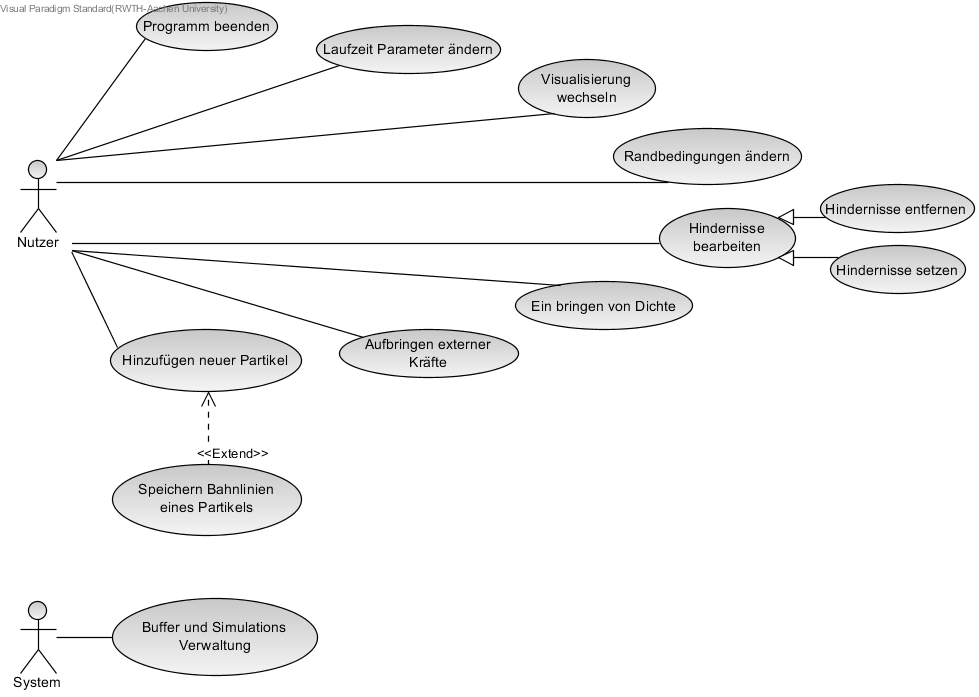
\includegraphics[width=1\linewidth]{images/Strom-UCD}
	\caption{Anwendungsfalldiagramm}
	\label{fig:use_case_diagram}
\end{figure}

\begin{enumerate}[font=\textbf]

 
    \item \textbf{Programm Beenden}
      \begin{description}[font=\normalfont\textit]
        \item[Ziel:] Beenden der Software
        \item[Einordnung:] Hauptfunktion
        \item[Vorbedingung:] Interface wird angezeigt
        \item[Nachbedingung:] Software beendet
        \item[Nachbedingung im Fehlerfall:] Software beendet 
        \item[Hauptakteure:] Nutzer
        \item[Nebenakteure:] Keiner
        \item[Ausl\"oser:] Nutzer m\"ochte Programm Beenden
        \item[Standartablauf:] ~
        \begin{enumerate}
          \item Nutzer dr\"uckt auf X oder beendet aus Terminal
          \item Programm schlie\ss{}t
        \end{enumerate}
        \item[Verzweigung:] ~
        \begin{itemize}
           \item Worker Thread noch aktiv
           \begin{itemize}
             \item Thread beenden
           \end{itemize}
         \end{itemize} 
    \end{description}
  \begin{figure}[H]
	  \centering
	  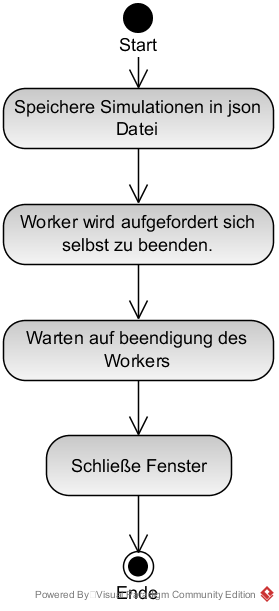
\includegraphics[width=0.3\linewidth]{images/Programm_beenden}
	  \caption{Aktivit\"atsdiagramm - Programm beenden}
	  \label{fig:activity_diagram_Programm beenden}
  \end{figure}

\begin{figure}[H]
	  \centering
	  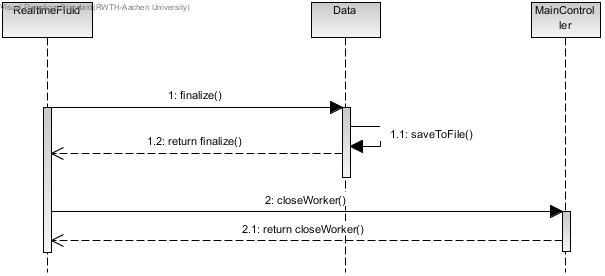
\includegraphics[width=\linewidth]{images/Programm_beenden_Sequence_Diagram.jpg}
	  \caption{Sequenzdiagramm - Programm beenden }
	  \label{fig:sequence_diagram_Programm_beenden}
  \end{figure}
  
     \item \textbf{Laufzeit Parameter ändern}
      \begin{description}[font=\normalfont\textit]
        \item[Ziel:] Parameter der Str\"omung w\"ahrend der Laufzeit des Programms verändern
        \item[Einordnung:] Hauptfunktion
        \item[Vorbedingung:] Interface wird angezeigt
        \item[Nachbedingung:] Interface wird angezeigt und Simulation l\"auft mit neuen Parametern
        \item[Nachbedingung im Fehlerfall:] Interface wird angezeigt 
        \item[Hauptakteure:] Nutzer
        \item[Nebenakteure:] System
        \item[Ausl\"oser:] Nutzer m\"ochte einen Str\"omungsparameter ver\"andern und navigiert zum entsprechenden Eingabefeld
        \item[Standartablauf:] ~
        \begin{enumerate}
          \item Auswahl eines Parameters im entsprechenden Feld
          \item Eingabe des Wertes
          \item System \"uberpr\"uft ob Wert im G\"ultigkeitsbereich ist
          \item Speicherung des neuen Wertes durch das System
        \end{enumerate}
                \item[Verzweigung:] ~
        \begin{itemize}
           \item Wert au\ss erhalb des G\"ultigkeitsbereiches
           \begin{itemize}
             \item System nimmt den Wert nicht an
           \end{itemize}
         \end{itemize} 
    \end{description}
  \begin{figure}[H]
	  \centering
	  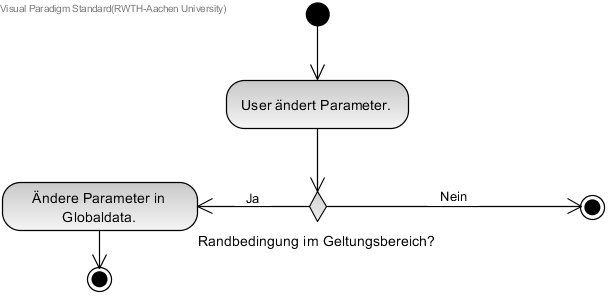
\includegraphics[width=\linewidth]{images/Laufzeit_Parameter}
	  \caption{Aktivit\"atsdiagramm - Laufzeit Parameter \"andern}
	  \label{fig:activity_diagram_Laufzeit Parameter}
  \end{figure}

\begin{figure}[H]
	  \centering
	  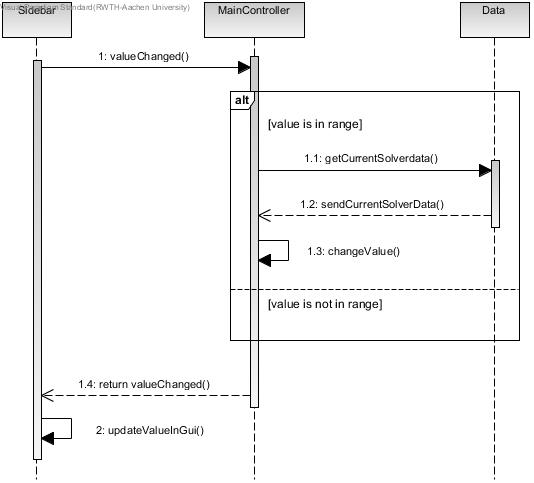
\includegraphics[width=\linewidth]{images/Laufzeit_Parameter_aendern_Sequence_Diagram.jpg}
	  \caption{Sequenzdiagramm - Laufzeit Parameter \"andern }
	  \label{fig:sequence_diagram_Laufzeit_Parameter_aendern}
  \end{figure}

      \item \textbf{Visualisierung wechseln}
      \begin{description}[font=\normalfont\textit]
        \item[Ziel:] Den Visualisierungsmodus der Simulation \"andern
        \item[Einordnung:] Hauptfunktion
        \item[Vorbedingung:] Interface wird angezeigt
        \item[Nachbedingung:] Interface wird angezeigt in der neuen Ansicht
        \item[Hauptakteure:] Nutzer
        \item[Nebenakteure:] System
        \item[Ausl\"oser:] Nutzer  m\"ochte Visualisierungsmodus wechseln
        \item[Standartablauf:] ~
        \begin{enumerate}
          \item Nutzer klickt auf den gew\"unschten Visualisierungsmodus-button
          \item System zeigt den gew\"unschten Visualisierungsmodus an
        \end{enumerate}
    \end{description}
  \begin{figure}[H]
	  \centering
	  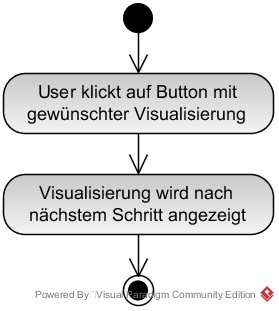
\includegraphics[width=0.4\linewidth]{images/Visualisierung}
	  \caption{Aktivit\"atsdiagramm - Visualisierung wechseln}
	  \label{fig:activity_diagram_Visualisierung wechseln}
  \end{figure}

\begin{figure}[H]
	  \centering
	  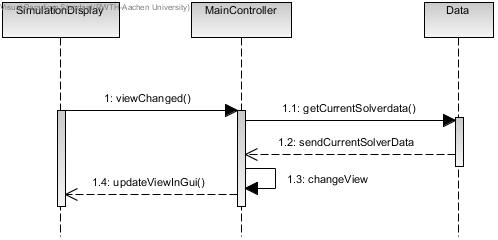
\includegraphics[width=\linewidth]{images/Visualisierung_wechseln_Sequence_Diagram.jpg}
	  \caption{Sequenzdiagramm - Visualisierung wechseln }
	  \label{fig:sequence_diagram_Visualisierung_wechseln}
  \end{figure}


  
    \item \textbf{Randbedingungen ändern}
      \begin{description}[font=\normalfont\textit]
        \item[Ziel:] Randbedingungen der Simulation ändern
        \item[Einordnung:] Hauptfunktion
        \item[Vorbedingung:] Interface wird angezeigt
        \item[Nachbedingung:] Interface wird angezeigt
        \item[Nachbedingung im Fehlerfall:] Interface wird angezeigt und Fehlermeldung wird ausgegeben
        \item[Hauptakteure:] Nutzer
        \item[Nebenakteure:] System
        \item[Ausl\"oser:] Nutzer m\"ochte die statischen Randbedinungen der Simulation ändern
        \item[Standartablauf:] ~
        \begin{enumerate}
          \item Nutzer w\"ahlt die zu \"andernde Bedingung aus und verändert sie
          \item System kontrolliert die Eingabe auf G\"ultigkeit
          \item System speichert die Randbedingung in den Buffer f\"ur den n\"achsten Simulationsneustart
        \end{enumerate}
        \item[Verzweigung:] ~
                \begin{itemize}
           \item Wert au\ss erhalb des G\"ultigkeitsbereiches
           \begin{itemize}
             \item System nimmt den Wert nicht an und zeigt Fehlermeldung in der Statusbar
           \end{itemize}
         \end{itemize} 
    \end{description}
  \begin{figure}[H]
	  \centering
	  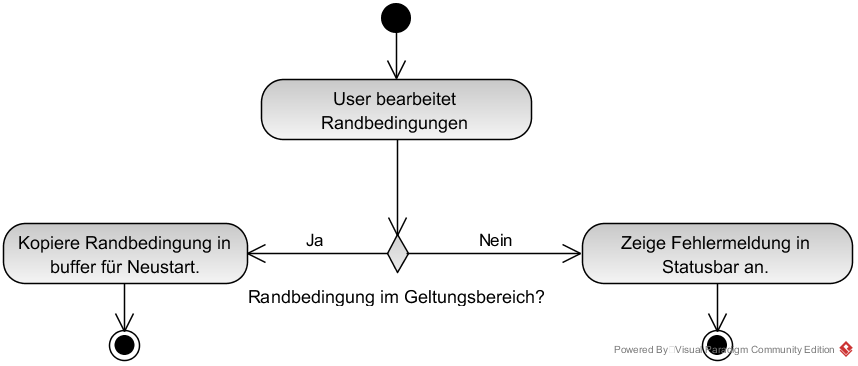
\includegraphics[width=\linewidth]{images/Randbedingung}
	  \caption{Aktivit\"atsdiagramm - Randbedingung \"andern}
	  \label{fig:activity_diagram_Randbedingung}
  \end{figure}

\begin{figure}[H]
	  \centering
	  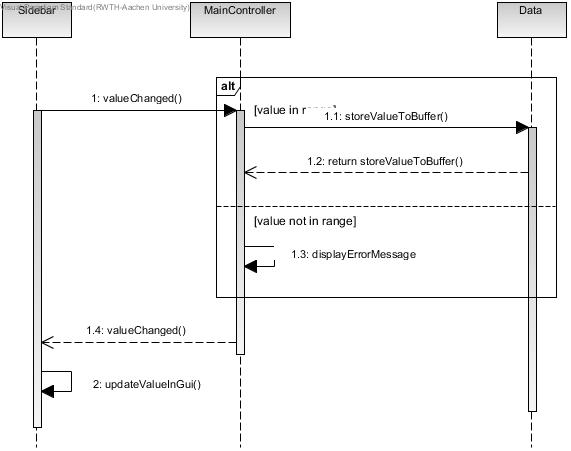
\includegraphics[width=\linewidth]{images/Randbedingungen_aendern_Sequence_Diagram.jpg}
	  \caption{Sequenzdiagramm - Randbedingungen \"andern }
	  \label{fig:sequence_diagram_Randbedingungen_aendern}
  \end{figure}
  
  
       \item \textbf{Hindernisse entfernen}
      \begin{description}[font=\normalfont\textit]
        \item[Ziel:] Ein Hindernis aus dem Str\"omungskanal löschen
        \item[Einordnung:] Hauptfunktion
        \item[Vorbedingung:] Interface wird angezeigt
        \item[Nachbedingung:] Interface wird angezeigt, Str\"omungskanal ist aktualisiert
        \item[Nachbedingung im Fehlerfall:] Interface wird angezeigt
        \item[Hauptakteure:] Nutzer
        \item[Nebenakteure:] System
        \item[Ausl\"oser:] Nutzer möchte ein Hindernis aus dem Str\"omungskanal löschen
        \item[Standartablauf:] ~
        \begin{enumerate}
          \item Nutzer klickt mit entsprechender Tastenkombination in das Programm.
          \item System überprüft ob die Position im Simulationsfeld ist
          \item Worker kontrolliert ob die Position gesperrt ist
          \item Speichern der Position im Buffer um dort das Hindernis im n\"achsten Schritt zu entfernen
        \end{enumerate}
        \item[Verzweigung:] ~
                        \begin{itemize}
           \item Position nicht im Str\"omungskanal
           \begin{itemize}
             \item System nimmt den Befehl nicht an
           \end{itemize}
         \end{itemize} 
                         \begin{itemize}
           \item Kein Hindernis an der Position vorhanden
           \begin{itemize}
             \item System nimmt den Befehl nicht an
           \end{itemize}
         \end{itemize} 
    \end{description}
  \begin{figure}[H]
	  \centering
	  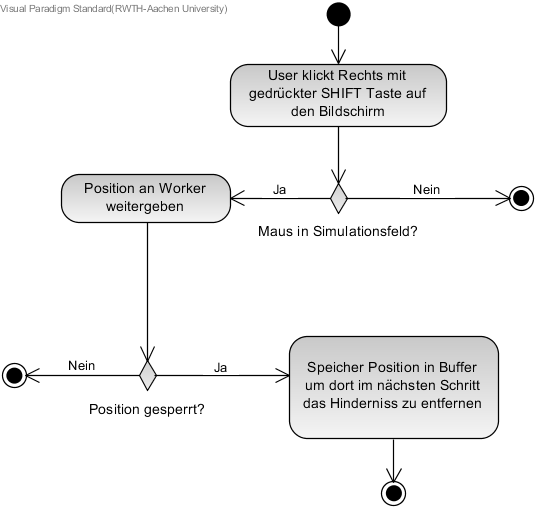
\includegraphics[width=0.8\linewidth]{images/Hindernisse_entfernen}
	  \caption{Aktivit\"atsdiagramm - Hindernisse entfernen}
	  \label{fig:activity_diagram_Hindernisse entfernen}
  \end{figure}
  
\begin{figure}[H]
	  \centering
	  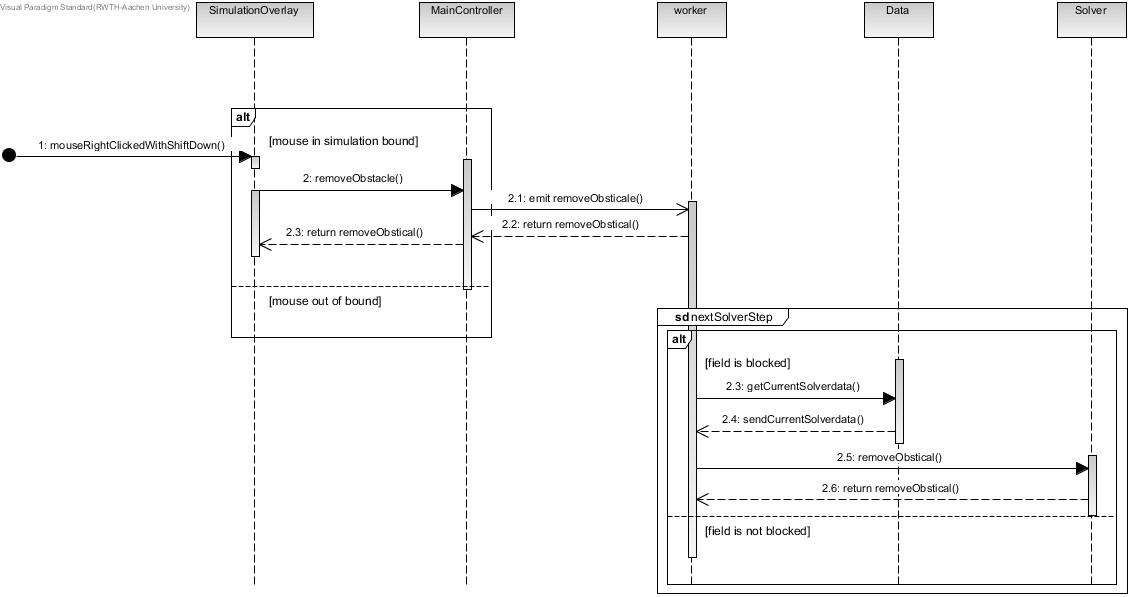
\includegraphics[width=\linewidth]{images/Hindernisse_entfernen_Sequence_Diagram.jpg}
	  \caption{Sequenzdiagramm - Hindernisse entfernen }
	  \label{fig:sequence_diagram_Hindernisse_entfernen}
  \end{figure}
  
    \item \textbf{Hindernisse setzen}
      \begin{description}[font=\normalfont\textit]
        \item[Ziel:] Ein Hindernis in den Strömungskanal setzen
        \item[Einordnung:] Hauptfunktion
        \item[Vorbedingung:] Interface wird angezeigt
        \item[Nachbedingung:] Interface wird angezeigt, Str\"omungskanal ist aktualisiert
        \item[Nachbedingung im Fehlerfall:] Interface wird angezeigt
        \item[Hauptakteure:] Nutzer
        \item[Nebenakteure:] System
        \item[Ausl\"oser:] Nutzer möchte ein Hindernis in den Str\"omungskanal setzen.
        \item[Standartablauf:] ~
        \begin{enumerate}
          \item Nutzer klickt mit entsprechender Tastenkombination in das Programm         
          \item System überprüft ob die Position im Simulationsfeld ist
          \item Worker kontrolliert ob die Position gesperrt ist
          \item Speichern der Position im Buffer um dort das Hindernis im n\"achsten Schritt hinzuzuf\"ugen
        \end{enumerate}
        \item[Verzweigung:] ~
           \begin{itemize}
           \item Position nicht im Str\"omungskanal
           \begin{itemize}
             \item System nimmt den Befehl nicht an
           \end{itemize}
         \end{itemize} 
                         \begin{itemize}
           \item Bereits ein Hindernis an der Position vorhanden
           \begin{itemize}
             \item System nimmt den Befehl nicht an
           \end{itemize}
         \end{itemize} 
    \end{description}
  \begin{figure}[H]
	  \centering
	  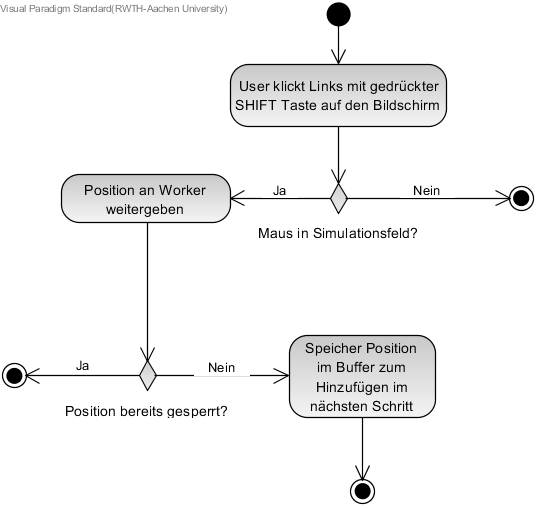
\includegraphics[width=0.8\linewidth]{images/Hindernisse_setzen}
	  \caption{Aktivit\"atsdiagramm - Hindernisse setzen}
	  \label{fig:activity_diagram_Hindernisse setzen}
  \end{figure}

\begin{figure}[H]
	  \centering
	  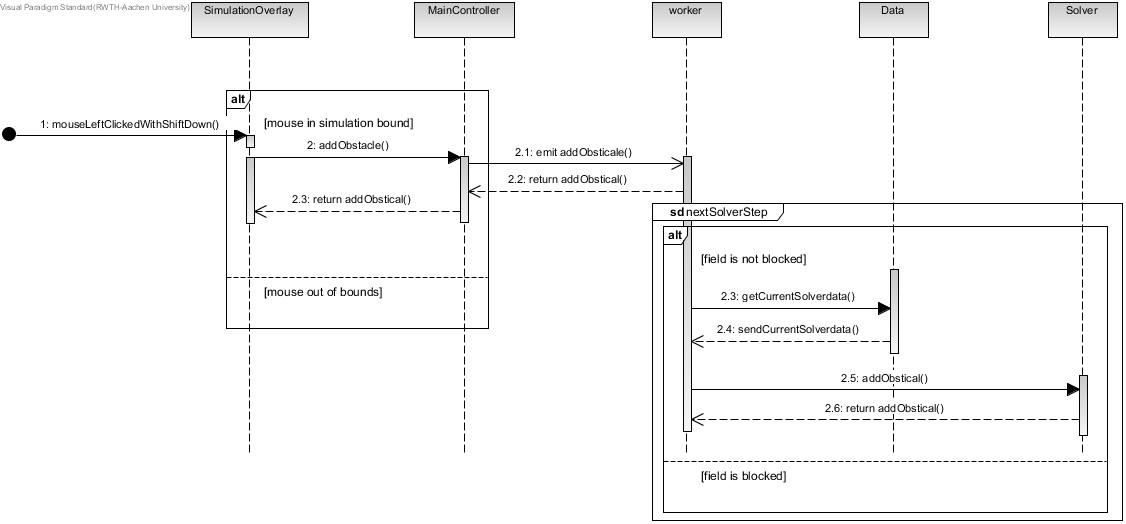
\includegraphics[width=\linewidth]{images/Hindernisse_setzen_Sequence_Diagram.jpg}
	  \caption{Sequenzdiagramm - Hindernisse setzen}
	  \label{fig:sequence_diagram_Hindernisse_setzen}
  \end{figure}
  
  
        \item \textbf{Einbringen von Dichte}
      \begin{description}[font=\normalfont\textit]
        \item[Ziel:] Dichte in den Str\"omungskanal setzen
        \item[Einordnung:] Hauptfunktion
        \item[Vorbedingung:] Interface wird angezeigt
        \item[Nachbedingung:] Interface wird angezeigt, Str\"omung ist aktualisiert
        \item[Nachbedingung im Fehlerfall:] Interface wird angezeigt
        \item[Hauptakteure:] Nutzer
        \item[Nebenakteure:] System
        \item[Ausl\"oser:] Nutzer m\"ochte die Verteilung von Dichte in der Str\"omung sehen.
        \item[Standartablauf:] ~
        \begin{enumerate}
          \item Nutzer macht Rechtsklick auf den Bildschirm
          \item System überpr\"uft ob die Stelle sich im Str\"omungskanal befindet
          \item System überpr\"uft ob man sich aktuell in der Density-Ansicht befindet.
          \item Speichern der Stelle im Buffer um dort im nächsten Schritt die Density einzusetzen
        \end{enumerate}
        \item[Verzweigung:] ~
           \begin{itemize}
           \item Position nicht im Str\"omungskanal
           \begin{itemize}
             \item System nimmt den Befehl nicht an
           \end{itemize}
         \end{itemize} 
          \begin{itemize}
           \item Nicht in der Density Ansicht
           \begin{itemize}
             \item System nimmt den Befehl nicht an
           \end{itemize}
         \end{itemize} 
    \end{description}
  \begin{figure}[H]
	  \centering
	  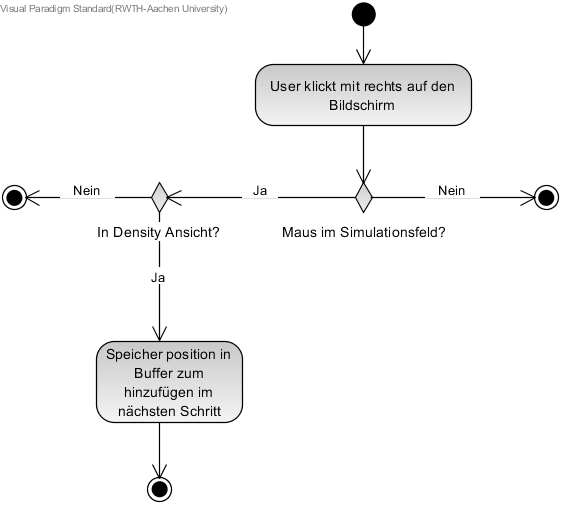
\includegraphics[width=0.8\linewidth]{images/dichte}
	  \caption{Aktivit\"atsdiagramm - Einbringen von Dichte}
	  \label{fig:activity_diagram_Einbringen von Dichte}
  \end{figure}

\begin{figure}[H]
	  \centering
	  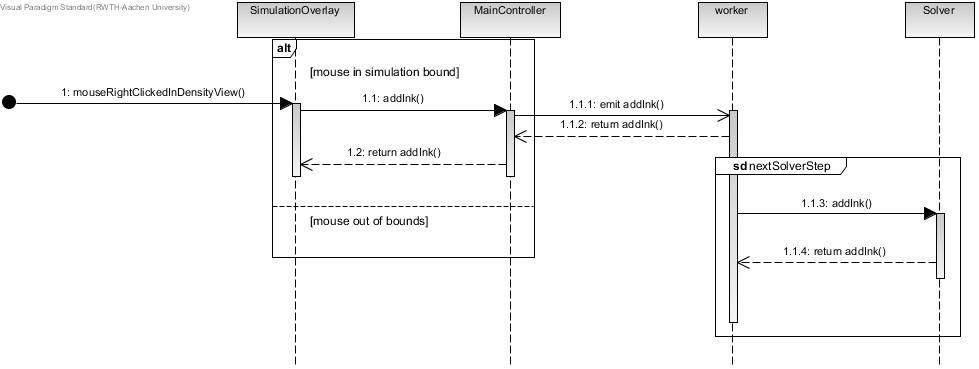
\includegraphics[width=\linewidth]{images/Einbringen_von_Dichte_Sequence_Diagram.jpg}
	  \caption{Sequenzdiagramm - Einbringen von Dichte}
	  \label{fig:sequence_diagram_Einbringen_von_Dichte}
  \end{figure}
  
          \item \textbf{Aufbringen externer Kr\"afte}
      \begin{description}[font=\normalfont\textit]
        \item[Ziel:] Mit externen Kr\"aften die Str\"omung beeinflussen 
        \item[Einordnung:] Hauptfunktion
        \item[Vorbedingung:] Interface wird angezeigt
        \item[Nachbedingung:] Interface wird angezeigt, Str\"omungsfeld ist aktualisiert
        \item[Nachbedingung im Fehlerfall:] Interface wird angezeigt
        \item[Hauptakteure:] Nutzer
        \item[Nebenakteure:] System
        \item[Ausl\"oser:] Nutzer möchte eine externe Kraft auf die Str\"omung anwenden
        \item[Standartablauf:] ~
        \begin{enumerate}
          \item Nutzer klickt mit entsprechender Tastenkombination auf den Bildschirm
          \item System überprüft ob die Klickposition im Simulationsfeld ist
          \item System überprüft mit welcher Taste gedrückt wurde
          \item System nimmt den Wert als Ausgangspunkt f\"ur die Richtungsvektorberechnung
          \item System wartet auf Nutzer bis er die Maus losl\"asst
          \item System speichert den Kraftvektor im Buffer um ihn im n\"achsten Schritt anzuwenden
        \end{enumerate}
        \item[Verzweigung:] ~
            \begin{itemize}
           \item Position nicht im Str\"omungskanal
           \begin{itemize}
             \item System nimmt den Befehl nicht an
           \end{itemize}
         \end{itemize} 
             \begin{itemize}
           \item Kein Linksklick
           \begin{itemize}
             \item System nimmt keinen Ausgangspunkt und bringt keine externe Kraft an
           \end{itemize}
         \end{itemize} 
    \end{description}
  \begin{figure}[H]
	  \centering
	  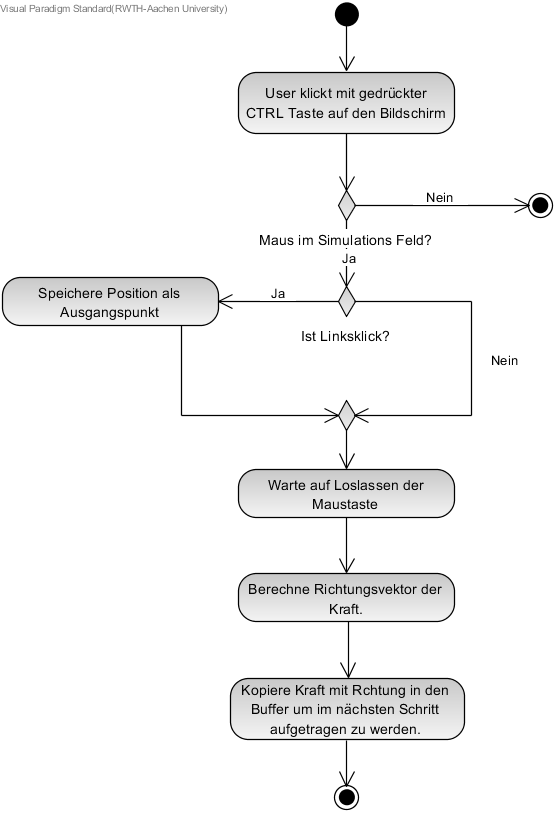
\includegraphics[width=0.8\linewidth]{images/extern_kraft}
	  \caption{Aktivit\"atsdiagramm - Aufbringen externer Kr\"afte}
	  \label{fig:activity_diagram_Aufbringen externer Kr\"afte}
  \end{figure}

\begin{figure}[H]
	  \centering
	  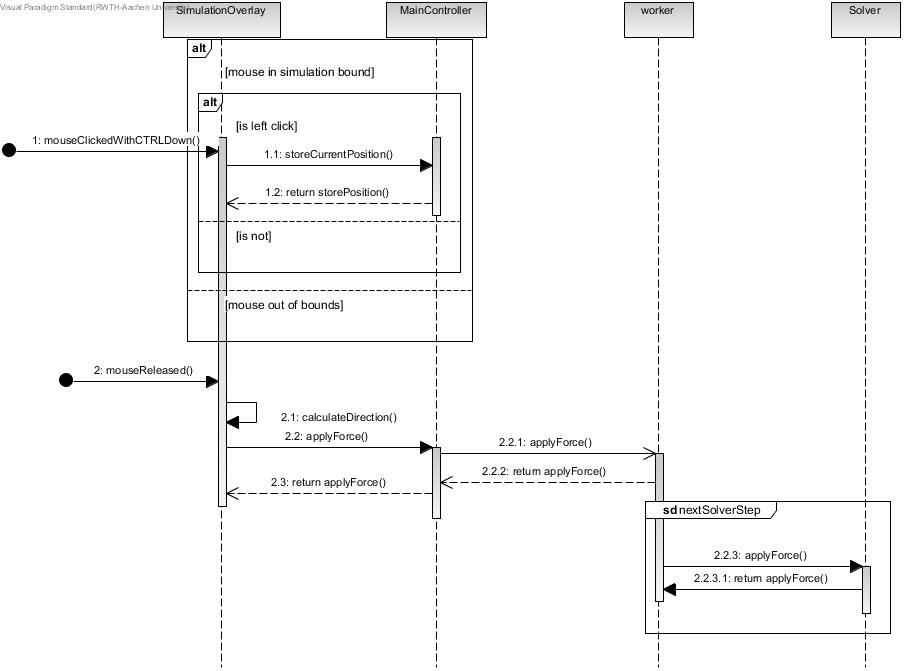
\includegraphics[width=\linewidth]{images/Aufbringen_externer_Kraefte_Sequence_Diagram.jpg}
	  \caption{Sequenzdiagramm -Aufbringen externer Kr\"afte}
	  \label{fig:sequence_diagram_Aufbringen_externer_Kraefte}
  \end{figure}
  
            \item \textbf{Hinzuf\"ugen neuer Partikel }
      \begin{description}[font=\normalfont\textit]
        \item[Ziel:] Ein Partikel in den Str\"omungskanal hinzuf\"ugen
        \item[Einordnung:] Hauptfunktion
        \item[Vorbedingung:] Interface wird angezeigt
        \item[Nachbedingung:] Interface wird angezeigt, Str\"omungskanal ist aktualisiert
        \item[Nachbedingung im Fehlerfall:] Interface wird angezeigt
        \item[Hauptakteure:] Nutzer
        \item[Nebenakteure:] System
        \item[Ausl\"oser:] Nutzer möchte ein Partikel in den Str\"omungskanal einf\"ugen
        \item[Standartablauf:] ~
        \begin{enumerate}
          \item Nutzer klickt mit gedr\"uckter Shift Taste auf den Bildschirm
          \item System überprüft ob die Stelle im Str\"omungskanal ist
          \item System kontrolliert ob es ein Linksklick war
          \item System speichert die Position Im Buffer damit dort im n\"achsten Schritt ein Teilchen hinzugef\"ugt werden kann
        \end{enumerate}
        \item[Verzweigung:] ~
                    \begin{itemize}
           \item Position nicht im Str\"omungskanal
           \begin{itemize}
             \item System nimmt den Befehl nicht an
           \end{itemize}
         \end{itemize} 
             \begin{itemize}
           \item Kein Linksklick
           \begin{itemize}
             \item System speichert ab der Position die Bahnlinien eines Partikels
           \end{itemize}
         \end{itemize} 
    \end{description}
  \begin{figure}[H]
	  \centering
	  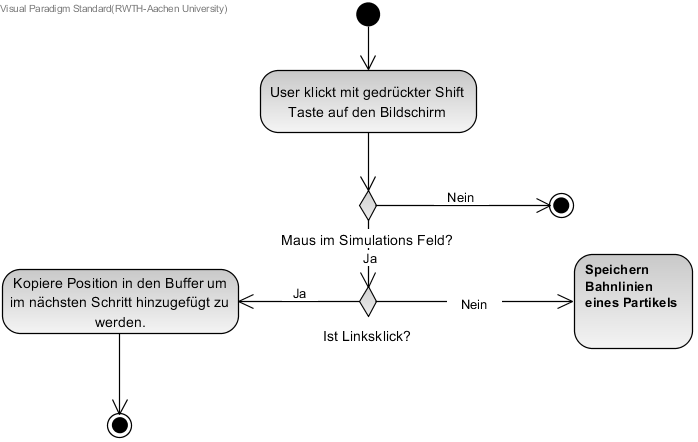
\includegraphics[width=\linewidth]{images/partikel_einfuegen}
	  \caption{Aktivit\"atsdiagramm - Hinzuf\"ugen neuer Partikel}
	  \label{fig:activity_diagram_Hinzuf\"ugen neuer Partikel}
  \end{figure}
  
  \begin{figure}[H]
	  \centering
	  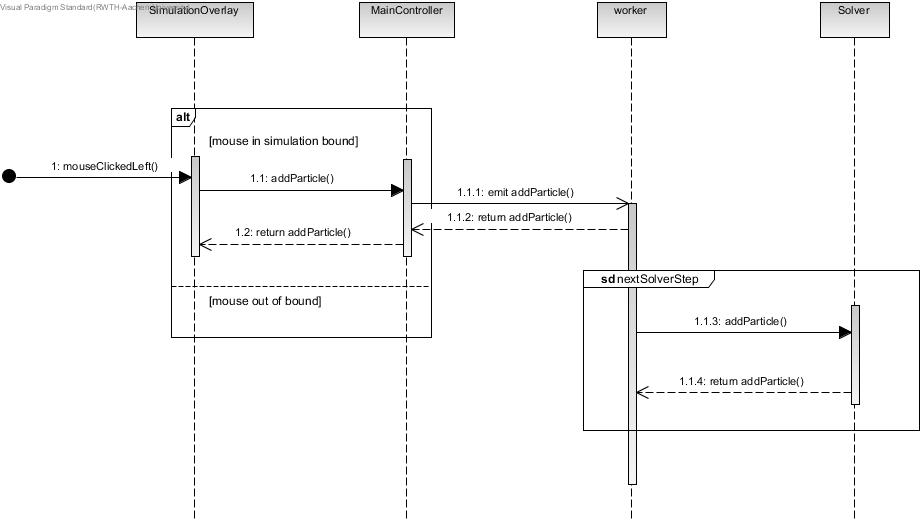
\includegraphics[width=\linewidth]{images/Hinzufuegen_neuer_Partikel_Sequence_Diagram.jpg}
	  \caption{Sequenzdiagramm - Hinzuf\"ugen neuer Partikel}
	  \label{fig:sequence_diagram_Hinzuf\"ugen_neuer_Partikel}
  \end{figure}


       \item \textbf{Speichern Bahnlinien eines Partikels }
      \begin{description}[font=\normalfont\textit]
        \item[Ziel:] Visualisierung der Bahnlinien eines Partikels
        \item[Einordnung:] Hauptfunktion
        \item[Vorbedingung:] Interface wird angezeigt
        \item[Nachbedingung:] Interface wird angezeigt, Str\"omungskanal ist aktualisiert
        \item[Nachbedingung im Fehlerfall:] Interface wird angezeigt
        \item[Hauptakteure:] Nutzer
        \item[Nebenakteure:] System
        \item[Ausl\"oser:] Nutzer möchte eine Bahnlinie in den Str\"omungskanal einf\"ugen
        \item[Standartablauf:] ~
        \begin{enumerate}
          \item Nutzer klickt f\"ugt Partikel mit linken Maustaste ein
   	 \item System speichert Position um ab dieser Position im n\"achsten Schritt eine Bahnlinie zu zeichnen
        \end{enumerate}
    \end{description}
  \begin{figure}[H]
	  \centering
	  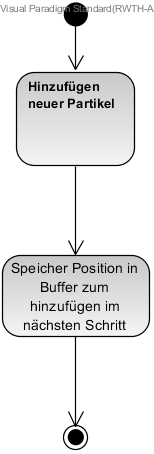
\includegraphics[width=0.25\linewidth]{images/Bahnlinien}
	  \caption{Aktivit\"atsdiagramm -Speichern Bahnlinien eines Partikels}
	  \label{fig:activity_diagram_Speichern Bahnlinien Partikell}
  \end{figure}

  \begin{figure}[H]
	  \centering
	  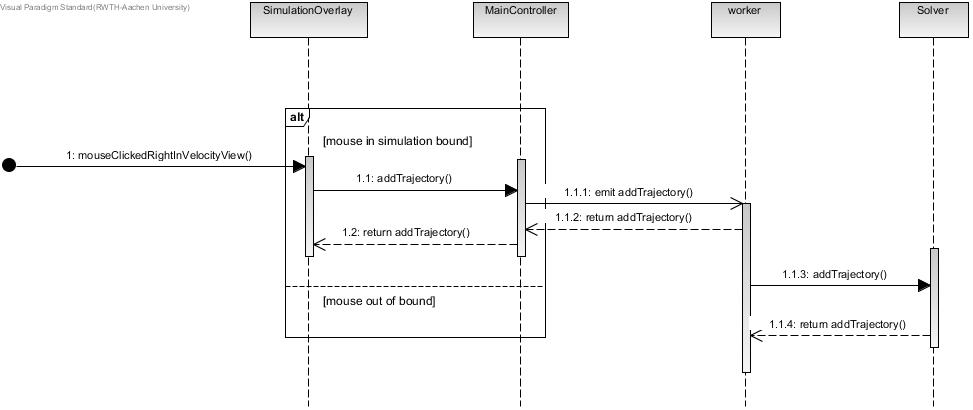
\includegraphics[width=\linewidth]{images/Speichern_Bahnlinien_eines_Partikels_Sequence_Diagram.jpg}
	  \caption{Sequenzdiagramm - Speichern Bahnlinien eines Partikels}
	  \label{fig:sequence_diagram_Speichern_Bahnlinien_eines_Partikels}
  \end{figure}
  
                \item \textbf{Buffer- und Simulationsverwaltung }
      \begin{description}[font=\normalfont\textit]
        \item[Ziel:] Berechnung und Verwaltung der Simulation
        \item[Einordnung:] Hauptfunktion
        \item[Vorbedingung:] Interface wird angezeigt
        \item[Nachbedingung:] Interface wird angezeigt, Str\"omungskanal ist aktualisiert
        \item[Nachbedingung im Fehlerfall:] Interface wird angezeigt
        \item[Hauptakteure:] Nutzer
        \item[Nebenakteure:] Keine
        \item[Ausl\"oser:] Die Simulation wird gestartet
        \item[Standartablauf:] ~
        \begin{enumerate}
          \item System startet neuen Simulationsschritt
          \item System holt sich die neuen Daten aus dem Buffer
          \item System l\"oscht die alten Daten
          \item System \"uberpr\"uft ob Simulation gewechselt werden soll
          \item System\"uberpr\"uft ob Simulation neu gestartet werden soll
	 \item  System berechnet die neuen Felder
          \item System aktualisiert den Str\"omungskanal in der GUI
        \end{enumerate}
        \item[Verzweigung:] ~
         \begin{itemize}
           \item Simulation soll gewechselt werden
           \begin{itemize}
             \item System holt sich die neue Simulation aus den Daten
           \end{itemize}
         \end{itemize} 
             \begin{itemize}
           \item Simulation soll neu gestartet werden
           \begin{itemize}
             \item System holt sich die neuen Randbedingungen aus dem Buffer und startet damit neu
           \end{itemize}
         \end{itemize} 
    \end{description}
  \begin{figure}[H]
	  \centering
	  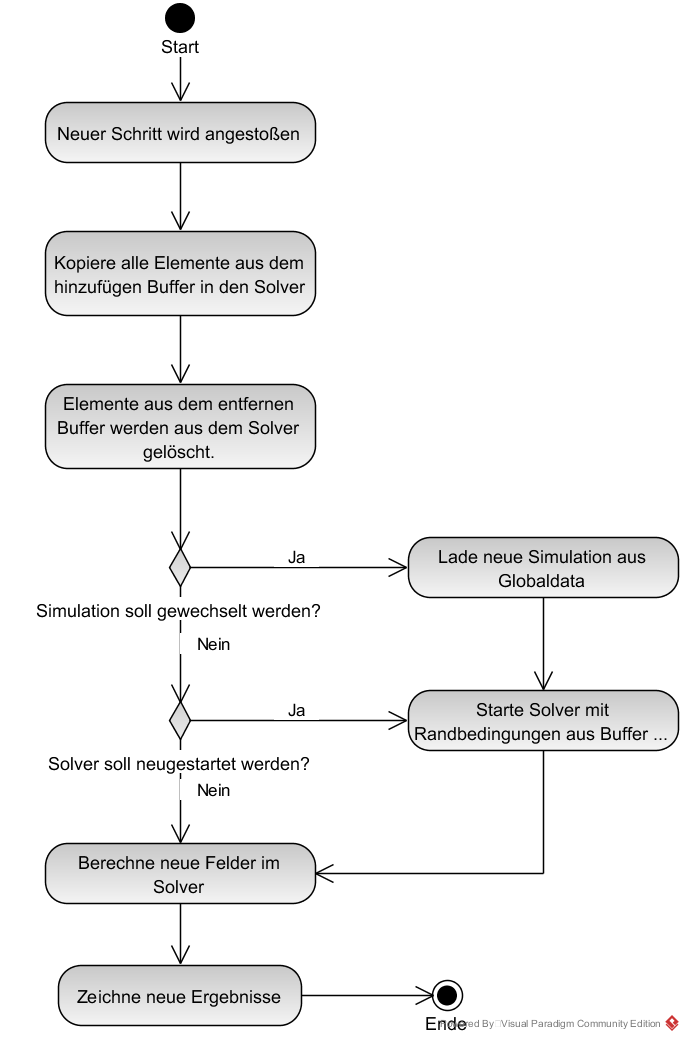
\includegraphics[width=0.8\linewidth]{images/Buffer_verwaltung}
	  \caption{Aktivit\"atsdiagramm - Buffer- und Simulationsverwaltung}
	  \label{fig:activity_diagram_Buffer und Simulationsverwaltung}
  \end{figure}

  \begin{figure}[H]
	  \centering
	  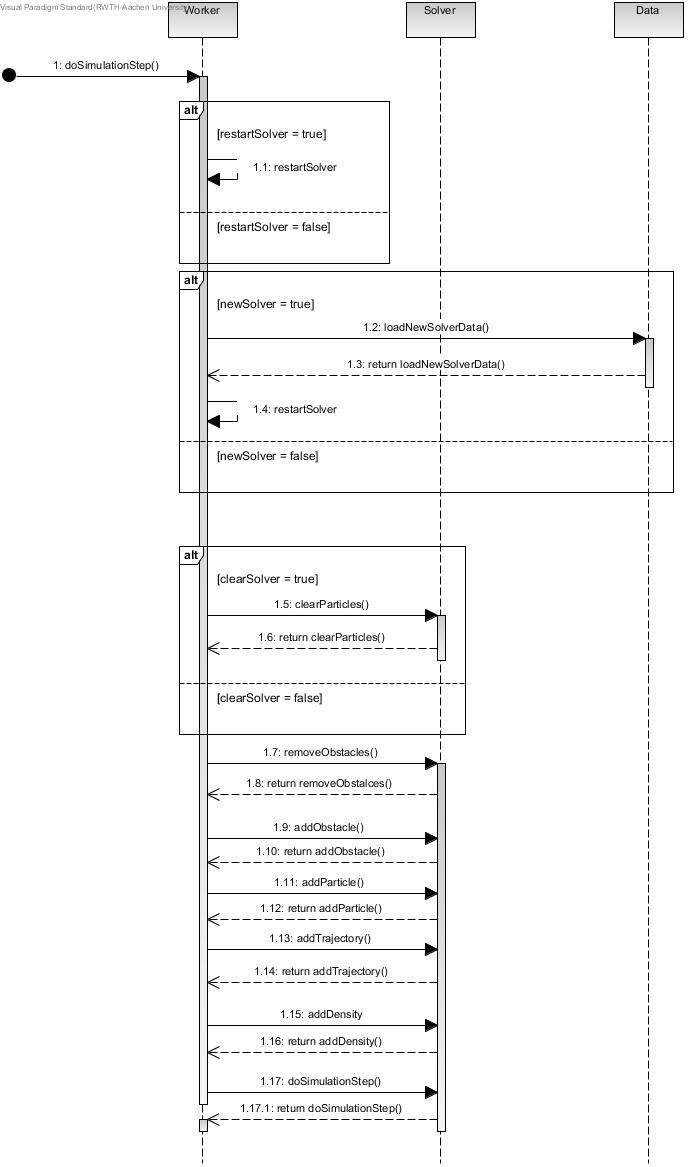
\includegraphics[width=\linewidth]{images/Buffer_und_Simulations_Verwaltung_Sequence_Diagram.jpg}
	  \caption{Sequenzdiagramm - Buffer und Simulations Verwaltung}
	  \label{fig:sequence_diagram_Buffer_und_Simulations_Verwaltung}
  \end{figure}
  
\end{enumerate}

\subsection{Systemanforderungen}  
\begin{description}[font=\normalfont\textit]
	\item[Funktionale Anforderungen:] ~
	\begin{itemize}
		\item Änderung von Strömungsparametern
		\item Änderung von Randbedingungen
		\item Setzen und L\"oschen von Hindernissen
		\item Zur\"ucksetzen der Simulation
		\item Auswahl der Gittergröße
		\item Hinzuf\"ugen von Partikeln und dessen Verlauf zeichnen (optional)
		\item Hinzuf\"ugen von Dichte
		\item Folgende Ansichten unterst\"utzen: Geschwindigkeits-, Druck-, Divergenz- und Dichteverteilungsfeld
		\item Externe Kr\"afte aufbringen
		\item Laden und Speichern von Simulationen
		\item Parallelisierung mit OpenMP 
	\end{itemize}
	\item[Nichtfunktionale Anforderungen:] ~
	\begin{itemize}
		\item C++ compiler: g++ (Version mindestens 5.2) oder clang (Version mindestens 3.5)
		\item cmake (Version mindestens 2.7)
		\item Externe Libraries:
			\begin{itemize}
				\item Boost
				\item Qt mit OpenGL (Version mindestens 5)
				\item Eigen (wird mitgeliefert)
			\end{itemize}
	\end{itemize}
	
	\item[Benutzbarkeitsanforderungen:] ~
	
	Das Programm soll auf dem Linux Betriebssystem laufen, unter anderem auf dem RWTH Cluster.
	
	\item[Performance:] ~
	
	Die Berechnung und Visualisierung der Strömung sollte sofort und durchgehend live geschehen. Das Programm soll auch noch performant auf normalen Computern laufen. Um dies zu erleichtern, benutzt das Programm die Open Multi-Processing library 	'omp.h'. Hiermit werden, wenn vorhanden, mehrere Kerne des Prozessors benutzt, um die Berechnungen durchzuf\"uhren.
	
	\item[Anzeige eines Userinterfaces:] ~
	
	Die verschiedenen Möglichkeiten des Nutzers mit der Software zu interagieren sollten ansprechend und einfach dargestellt sein. 
	
\end{description}


\section{Begriffsanalyse}

\begin{description}[font=\normalfont\textbf]
	\item[Klassenkandidaten:] ~
	\begin{itemize}
		\item Solver(L\"osen von Gleichungen) 
		\item MainController (MVC)
		\item Worker (Realisierung von Mulithreading)
		\item SimulationDisplay (Visualisierung mit Qt und OpenGL)
		\item SimulationOverlay (Eingaben in die Simulation per Maus)
		\item Parameterwahl (Textfeld oder Spinner) 
		\item Data (Laden und Speichern von Simulationen)
		\item Pr\"ufen auf valide Eingaben durch Qt
		\item AspectRatioHolder (Beibehaltung des Seitenverh\"ltnisses)
		\item ResourceManager (Externe speicherung von Anzeigetext)
		\item Sidebar (Eingabefelder und Anzeigen)
		\item StorageBar (Buttons)		
		\item Statusbar (Aktuelle Informationen)
	\end{itemize}
\end{description}

\chapter{Entwurf}

Aus reinem Quellcode einen Programmablauf und insbesondere die Beziehungen der einzelnen Klassen zu verstehen, kann sehr komplex sein. Deshalb benutzen wir Paket- und Klassendiagramme um einen grafischen Überblick zu ermöglichen.

\section{Pakete}

Das Pakete f\"ur das GUI ergibt sich aus dem von uns verwendeten Model-View-Controller (MVC) Konzept. Die Berechnung der Simulation erfolgen \"uber das solver Paket, welches wiederum das Paket basic inkludiert. 

In dem \textit{basic} Paket sind mit Hilfe der Eigen Library grunds\"atzliche Operationen sowie getter und setter f\"ur die von uns verwendeten Matrizen definiert. In dem \textit{solver} Paket sind einmal die innerhalb der Simulation verwendeten Variablen definiert, zum anderen die von uns f\"ur die Simulation benutzten numerischen Verfahren. 
Das GUI verwendet drei Pakete:
\begin{itemize}
\item Model
\item View
\item Controller
\end{itemize}

Hier wird das klassische MVC Konzept verwendet.

\section{Abstrakte Datentypen}

Unsere Software benutzt keine Abstrakten Datentypen. Der Code wurde aber so geschrieben, dass vor allem der Solver sehr leicht zu einem abstrakten Datentyp umgewandelt werden k\"onnte.  Das war aber vom Betreuer nicht gew\"unscht.

\section{Klassen}
\label{sec:Klassenkapitel}

Da das gesamte Klassendiagramm zu groß ist f\"ur ein einziges Diagramm , zeigen wir die Klassendiagramme der einzelnen Programmmodule. Bei dem Modul \textit{Model} ist zudem noch seine Beziehung zum Solver dargestellt.

\begin{figure}[H]
	\centering
	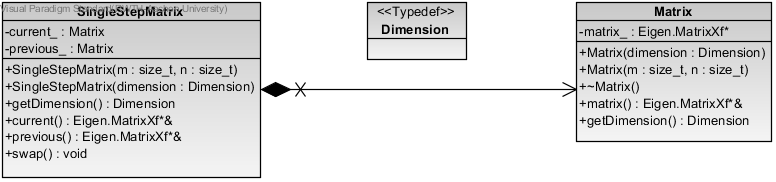
\includegraphics[width=\textwidth]{images/class-basic}
	\caption{Klassendiagramm basic}
	\label{fig:class-basic}
\end{figure}

\begin{figure}[H]
	\centering
	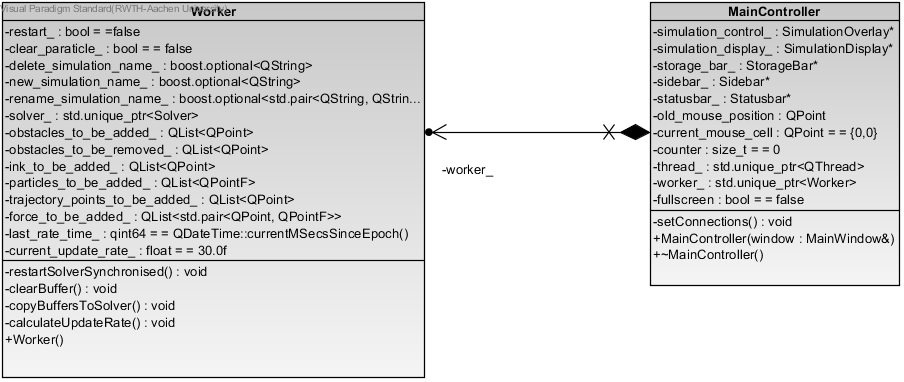
\includegraphics[width=\textwidth]{images/class-controller}
	\caption{Klassendiagramm Controller}
	\label{fig:class-controller}
\end{figure}

\begin{figure}[H]
	\centering
	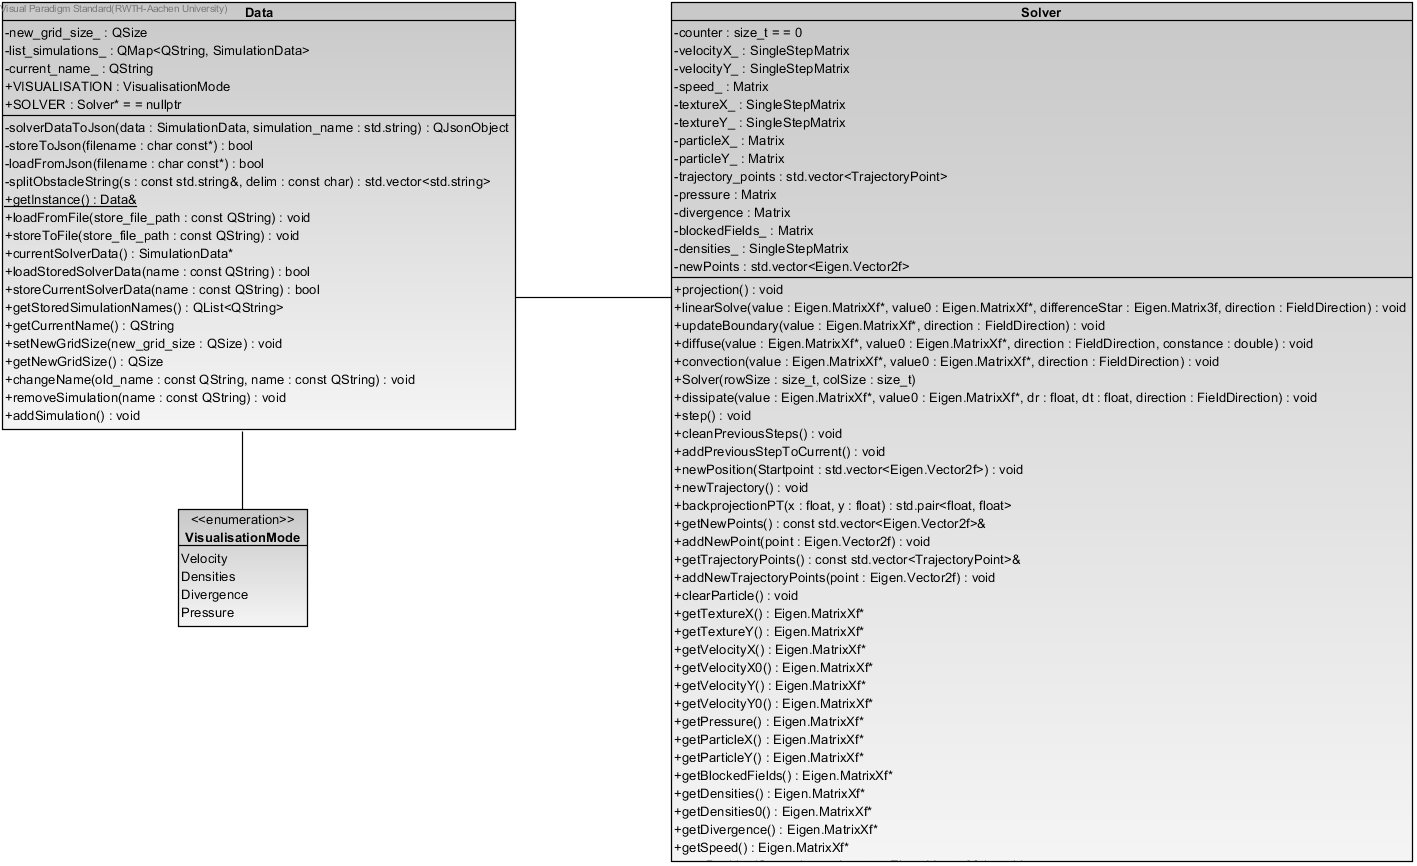
\includegraphics[width=\textwidth]{images/class-model}
	\caption{Klassendiagramm Model, mit Beziehung zum Solver}
	\label{fig:class-model}
\end{figure}

\begin{figure}[H]
	\centering
	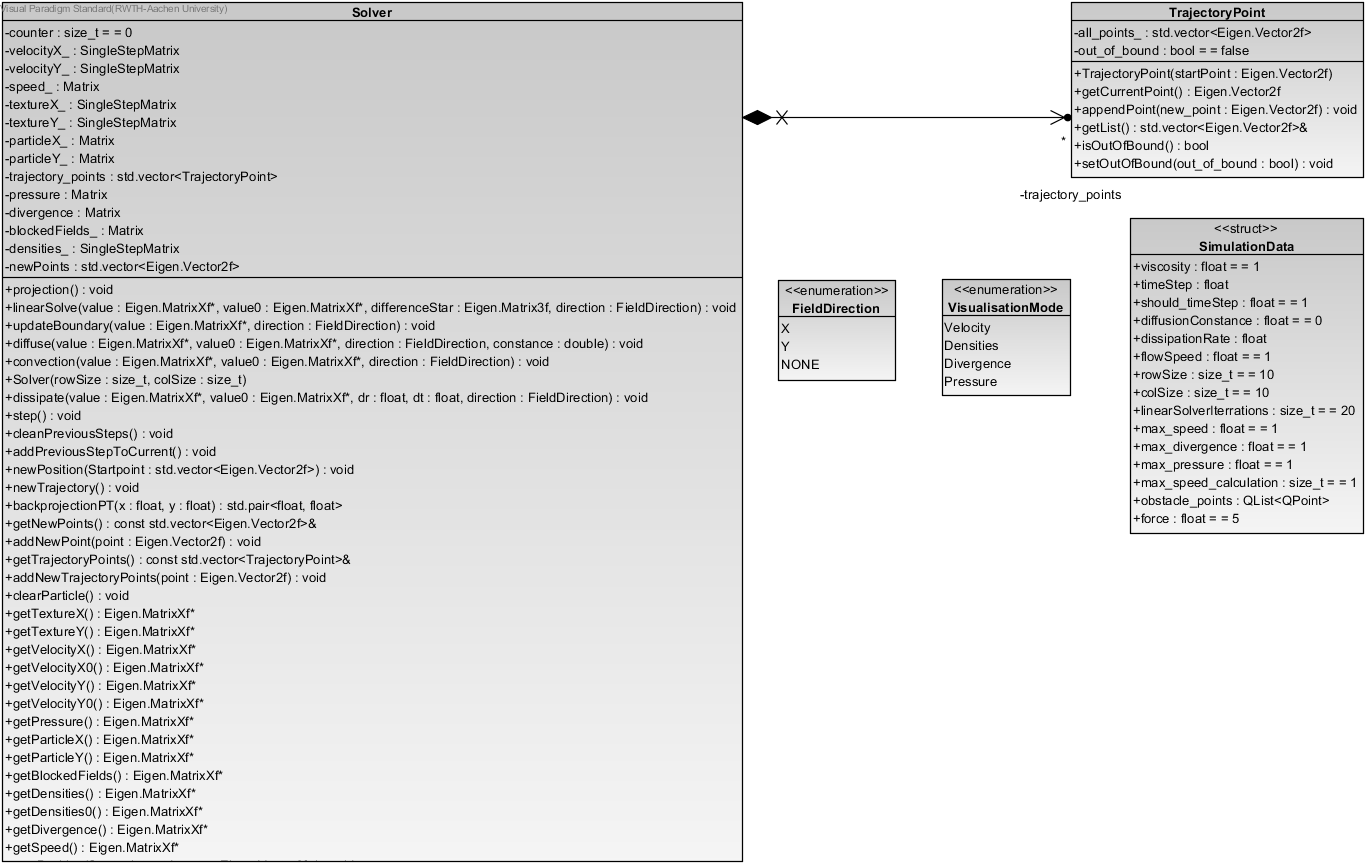
\includegraphics[width=\textwidth]{images/class-solver}
	\caption{Klassendiagramm Solver}
	\label{fig:class-solver}
\end{figure}

\begin{figure}[H]
	\centering
	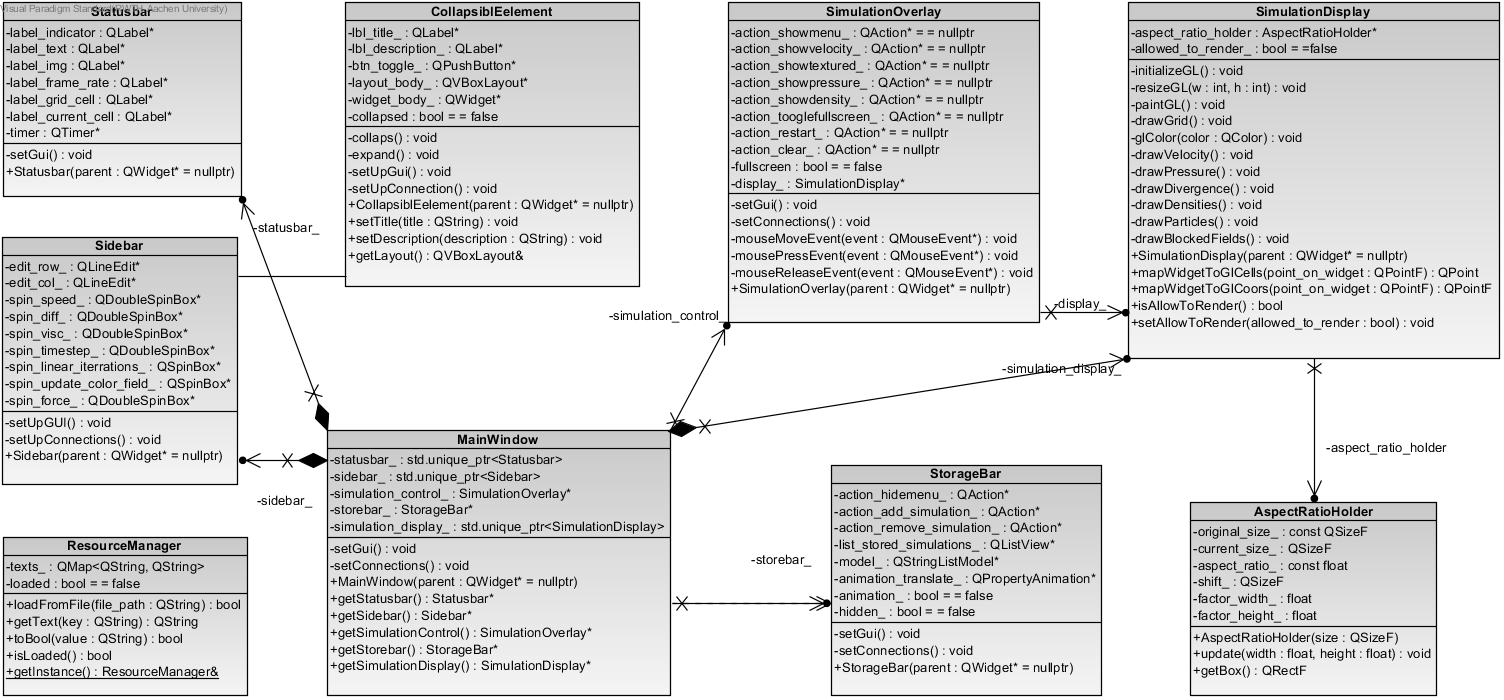
\includegraphics[width=\textwidth]{images/class-view}
	\caption{Klassendiagramm View}
	\label{fig:class-view}
\end{figure}




\chapter{Benutzerdokumentation}

Dokumentationen sind sehr wichtig, nicht  nur für die Entwickler, sondern auch für die Anwender. Programme sollten so intuitiv wie möglich sein. Trotzdem ist es sinnvoll ein Handbuch zu haben. Hier Dokumentieren wir die Anwendung unserer Software und geben Beispiele für die Nutzung.

\section{Installation}

F\"ur eine ausf\"urliche Installationsanleitung siehe \textit{code/README.md}

\section{Beispielsitzung und Bedienungsanleitung}

Es folgt nun eine kurze Beispielsitzung die auch als Bedienungsanleitung dient. Nach dem \"Offnen des Programms erscheint folgende GUI:

\begin{figure}[H]
	\centering
	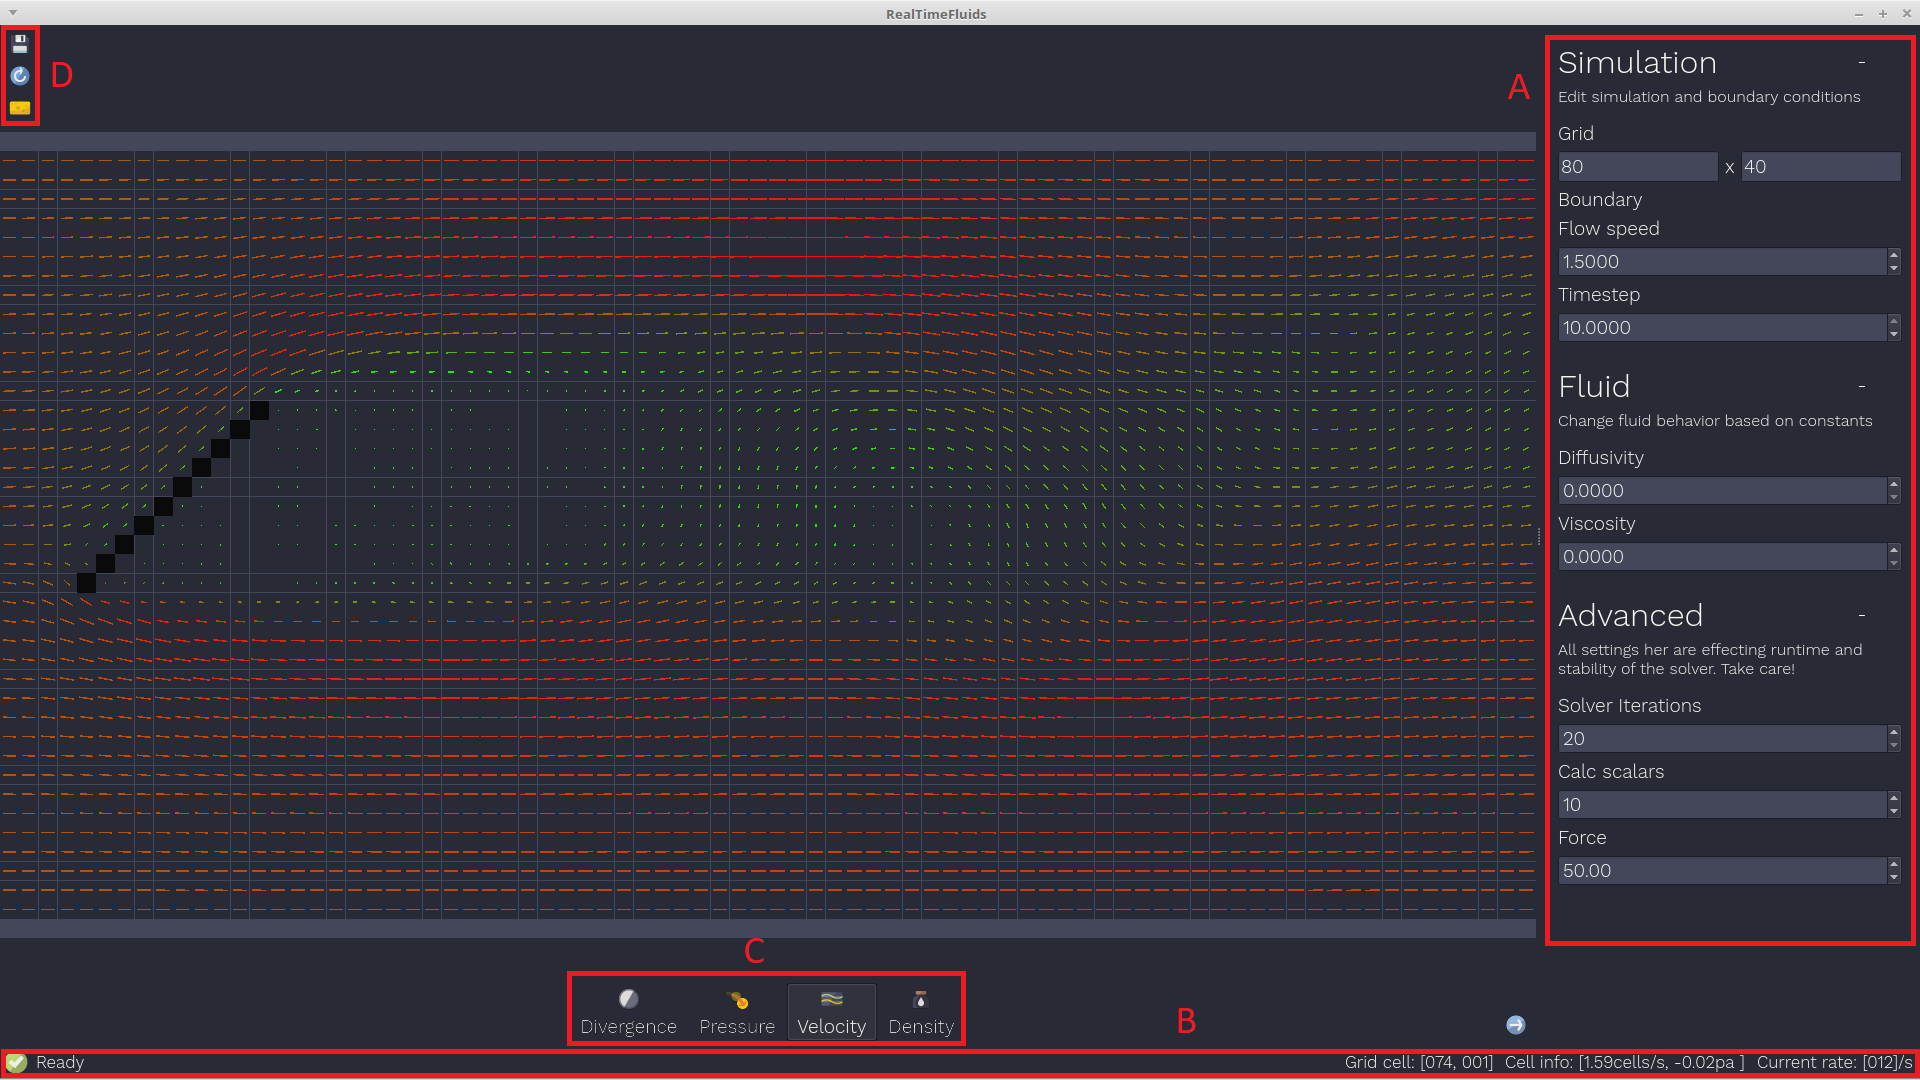
\includegraphics[width=\textwidth]{images/Startup.png}
	\caption{GUI nach dem Start}
	\label{fig:GUI_Start}
\end{figure}

Zuerst erfolgt eine kurze Zusammenfassung, danach wird im Detail auf die einzelnen Komponenten eingegangen.

Das \textit{Feld A} ist die sogenannte Sidebar. Hier werden die die Anfangswerte sowie Randbedingungen der Simulation angezeigt.

Das \textit{Feld B} ist die Statusbar. Hier wird der aktuelle Status der Simulation sowie gewisse Informationen \"uber das aktuell mit der Maus ausgew\"ahlte Feld des Str\"omungsfeldes angezeigt.

Im \textit{Feld C} k\"onnen die verschiedenen Ansichten der Simulation ausgew\"ahlt werden.

Durch den obersten Knopf in \textit{Feld D} gelangt man in das Menü zum Laden und Speichern von Simulationen. Die unteren beiden Kn\"opfe werden zum neu Starten und Zur\"ucksetzen der Simulation benutzt.

\subsection{Ansichtsfelder}

Der Benutzer kann unterhalb des Str\"omungskanals zwischen vier verschiedenen Ansichten wechseln:
\begin{figure}[H]
	\centering
	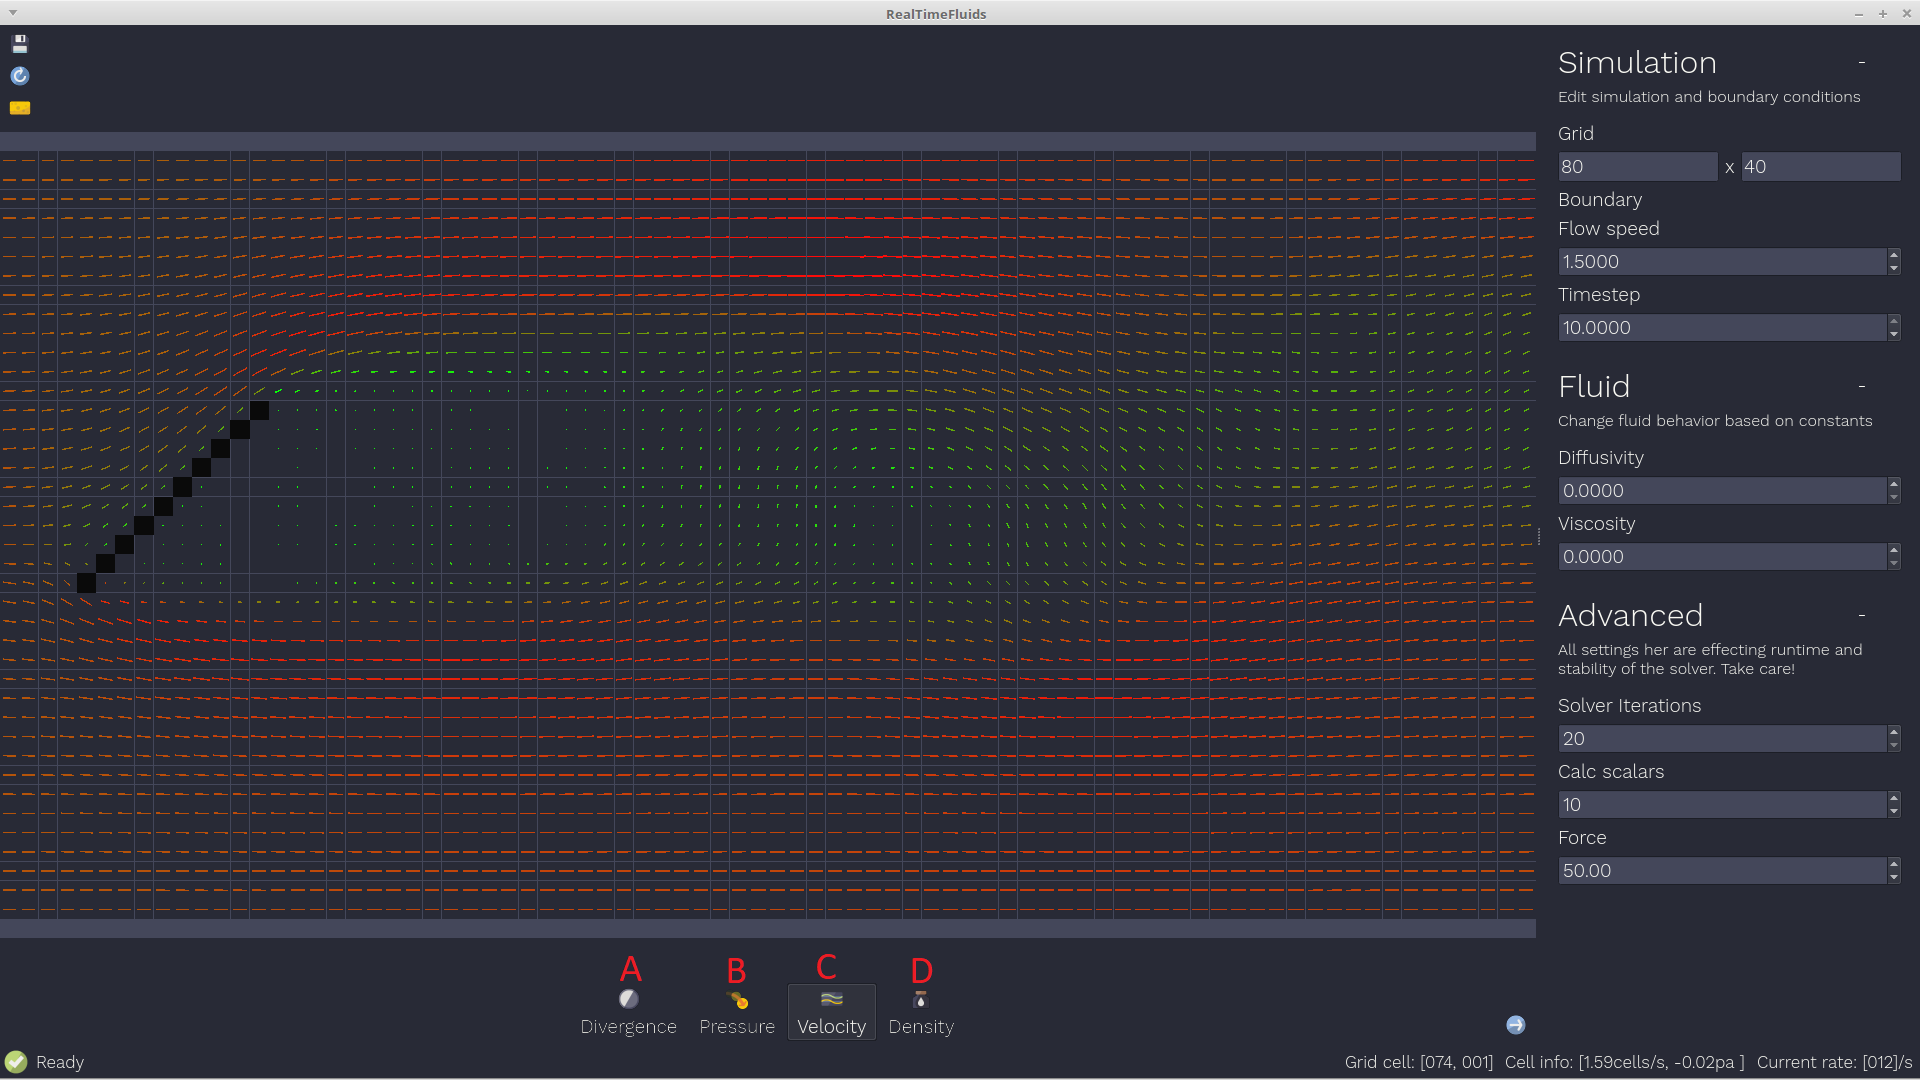
\includegraphics[width=\textwidth]{images/Field_View.png}
	\caption{Ansichten unterschiedlicher Felder}
	\label{fig:Ansichten_Felder}
\end{figure}

\renewcommand{\theenumi}{\Alph{enumi}}
\begin{enumerate}

\newpage

\item \textit{Divergenzfeld}

Das Divergenzfeld zeigt die G\"ute der Simulation. Die Divergenz berechnet sich aus den einzelnen Ein- und Ausfl\"ussen des Fluids in den jeweiligen Feldern.

\begin{figure}[H]
	\centering
	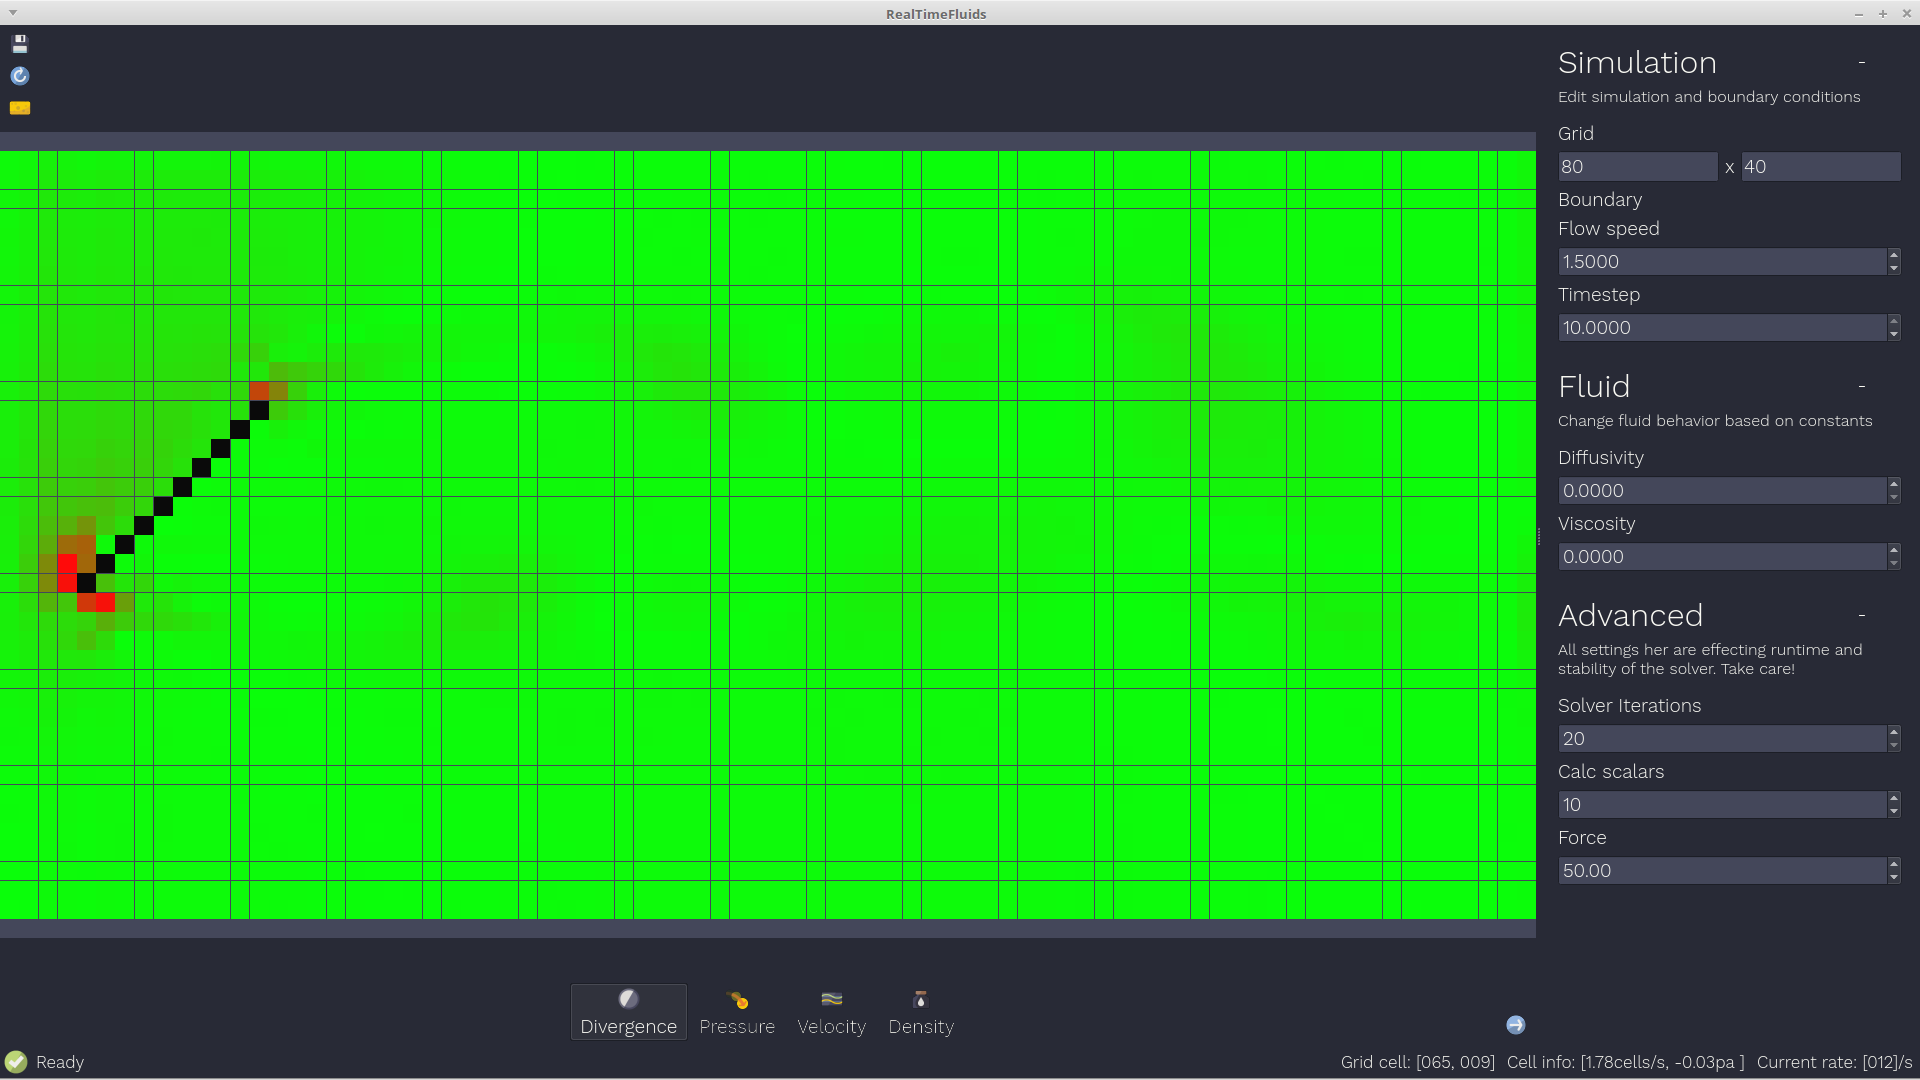
\includegraphics[width=\textwidth]{images/Divergence_Field.png}
	\caption{Divergenzfeld}
	\label{fig:Divergenzfeld}
\end{figure}

\item \textit{Druckfeld}

Das Druckfeld zeigt die verschiedenen Druckgebiete innerhalb des Str\"omungskanals. Diese Ansicht wird erst relevant, sobald man Hindernisse hinzugef\"ugt hat. Der Druck der mit dem Mauszeiger ausgew\"ahlten Zelle wird in der Statusbar in Zahlen angezeigt. Dabei handelt es sich um die Einheit Pascal.

\begin{figure}[H]
	\centering
	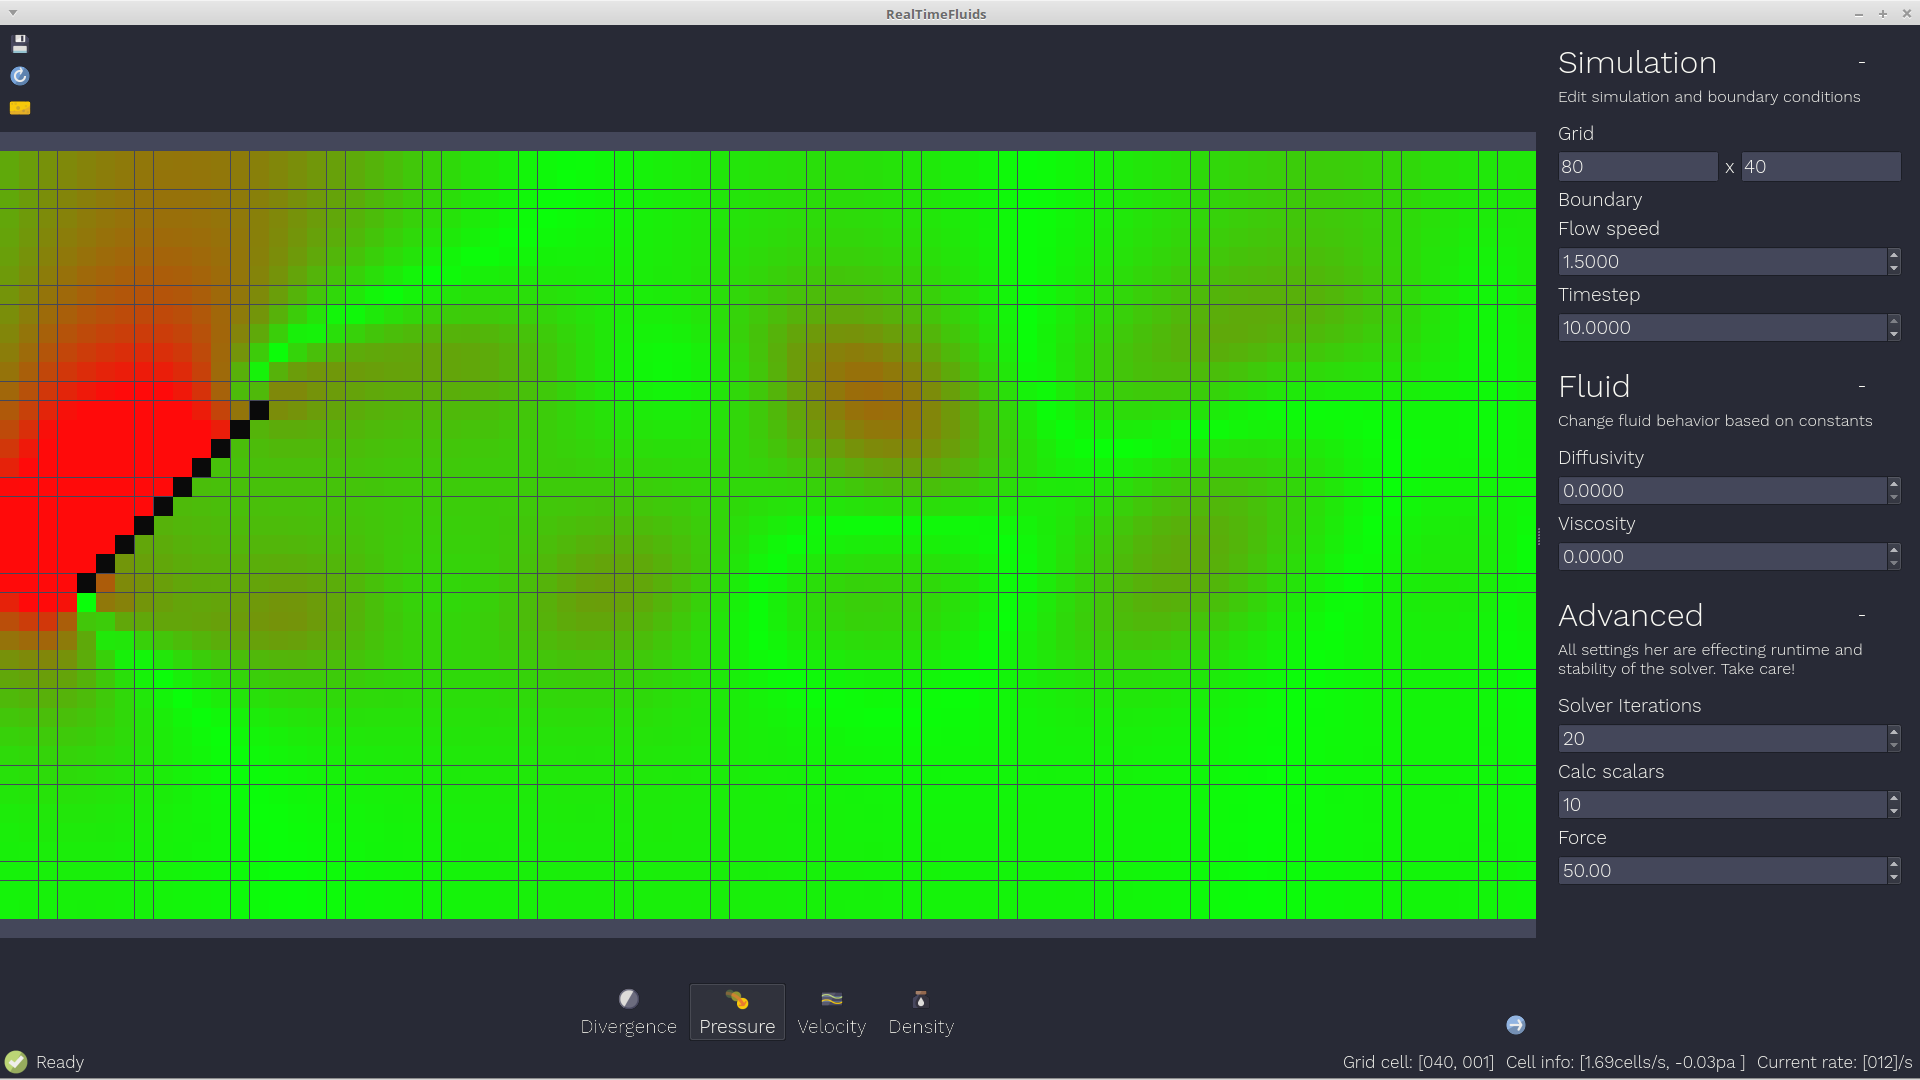
\includegraphics[width=\textwidth]{images/Pressure_Field.png}
	\caption{Druckfeld}
	\label{fig:Druckfeld}
\end{figure}

\item \textit{Geschwindigkeitsfeld}

Das Geschwindigkeitsfeld zeigt die Richtungsvektoren des Stroms innerhalb jeder Zelle. Anhand der Farbe und L\"ange der Vektoren ist zu erkennen, wie schnell das Fluid durch die jeweiligen Zellen flie\ss t. Die Visualisierung wird in Falschfarben dargestellt. Die Geschwindigkeit der mit dem Mauszeiger ausgew\"ahlten Zelle wird in der Statusbar in Zahlen angezeigt. Dabei handelt es sich um die Einheit $\frac{cells}{s}$.

\begin{figure}[H]
	\centering
	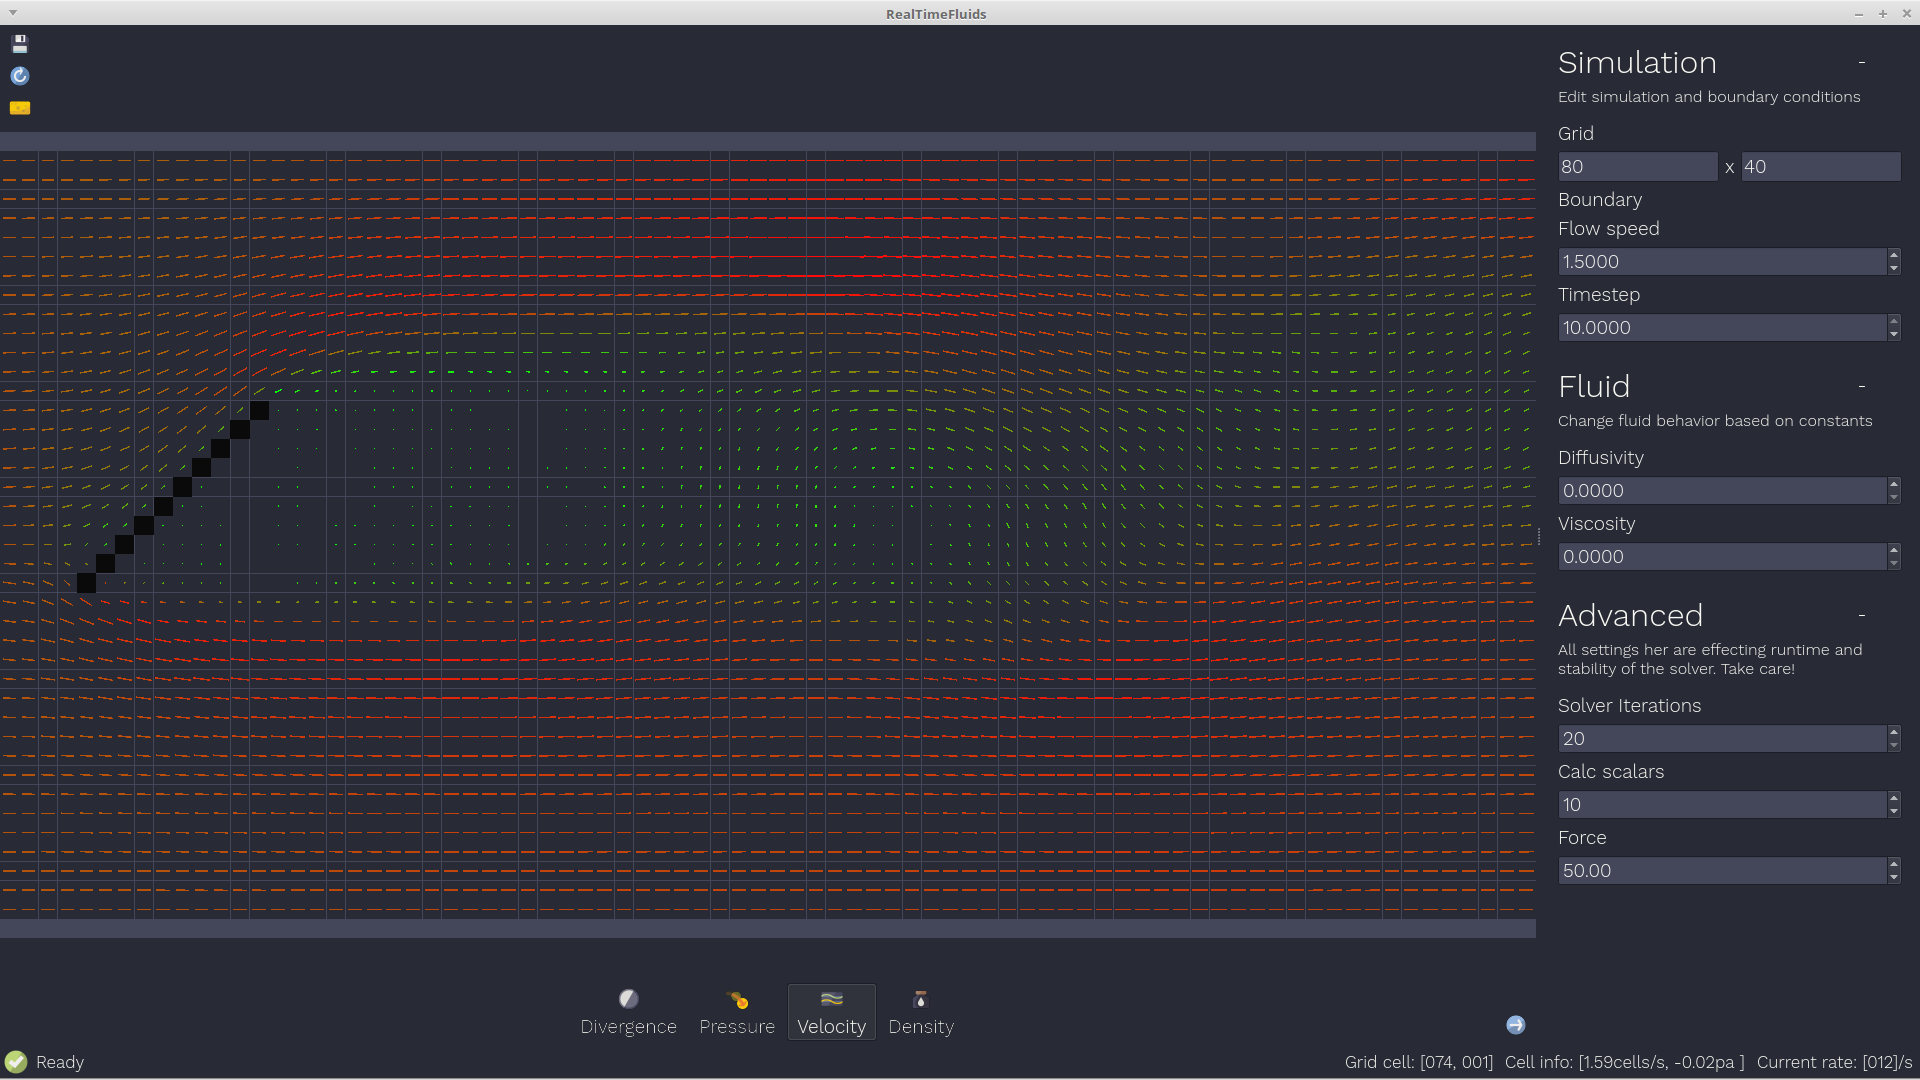
\includegraphics[width=\textwidth]{images/Velocity_Field.png}
	\caption{Geschwindigkeitsfeld}
	\label{fig:Geschwindigkeitsfeld}
\end{figure}

\item \textit{Dichteverteilungsfeld}

Das Dichteverteilungsfeld zeigt, wie der Name impliziert, die Verteilung der Dichte von hinzugef\"ugter Tinte im Str\"omungskanal.

\begin{figure}[H]
	\centering
	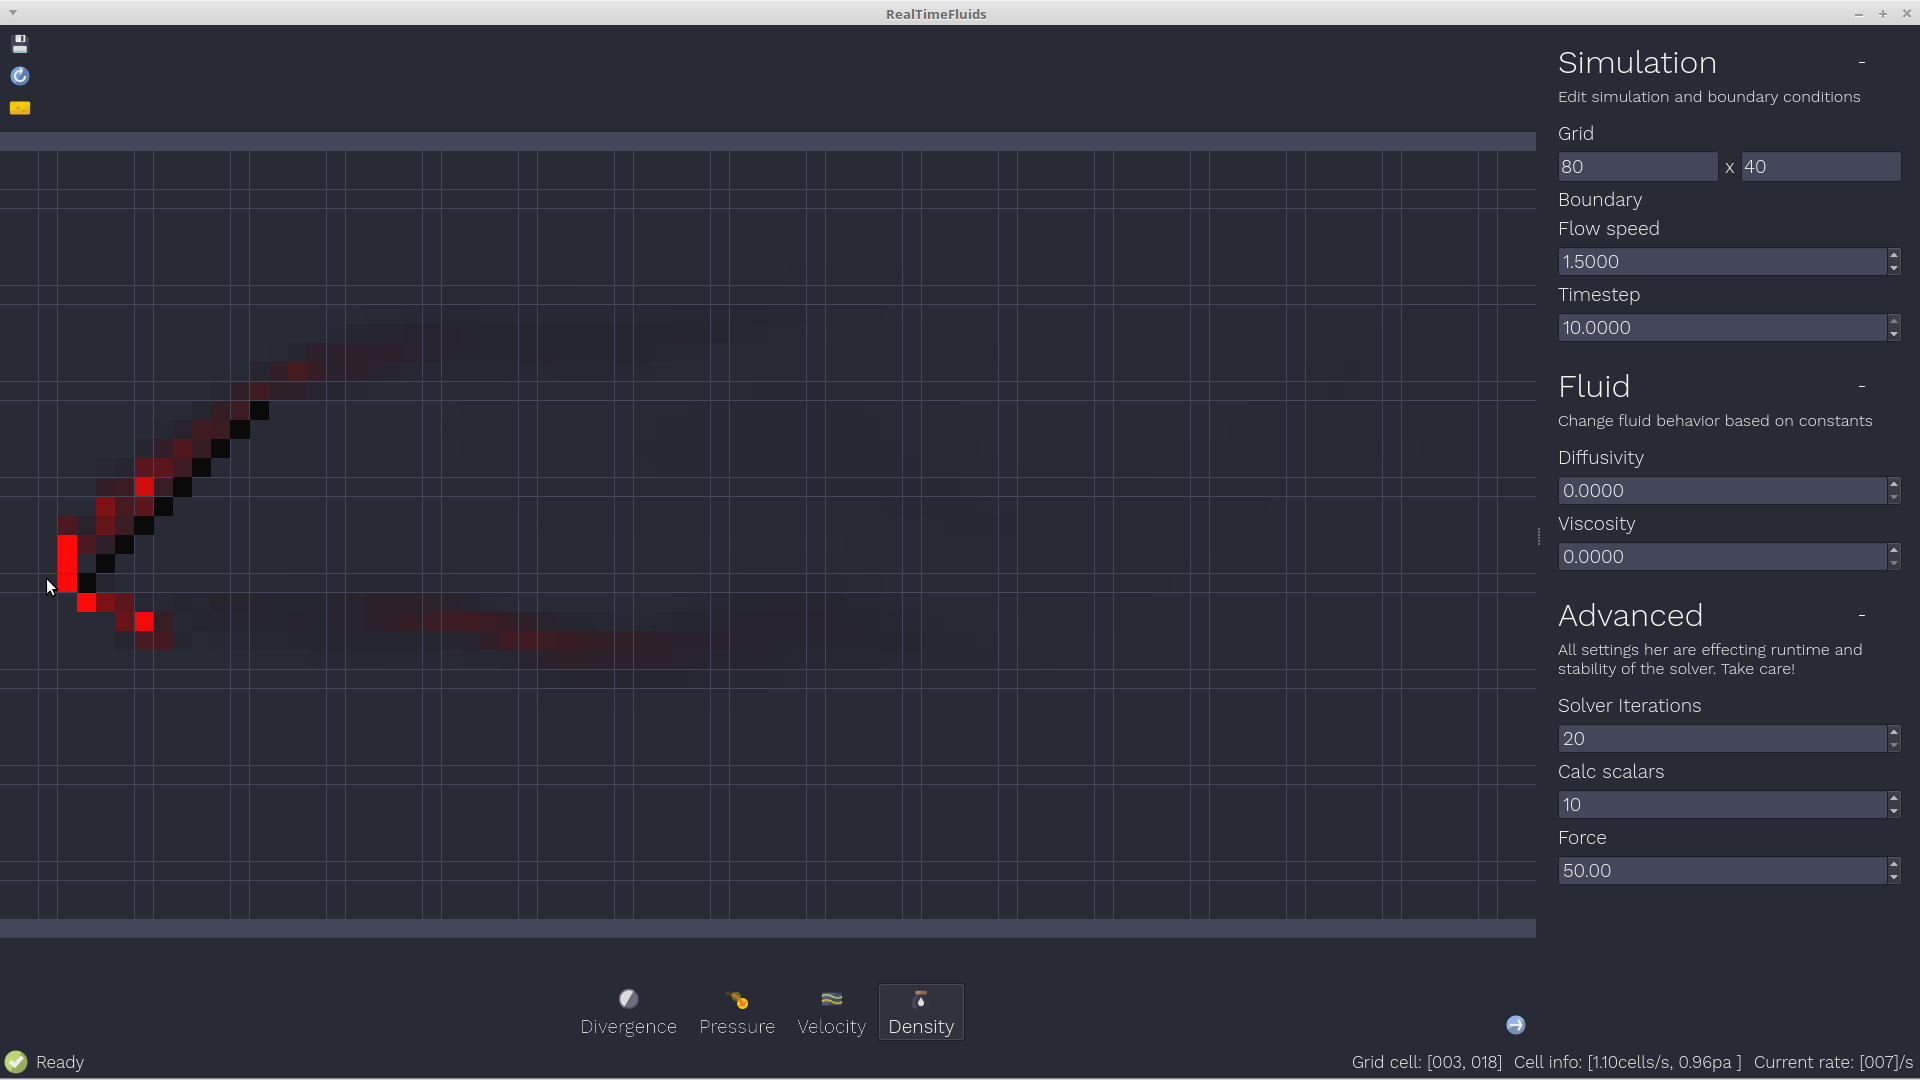
\includegraphics[width=\textwidth]{images/Density_Field.png}
	\caption{Dichteverteilungsfeld}
	\label{fig:Dichteverteilungsfeld}
\end{figure}
\end{enumerate}

\renewcommand{\theenumi}{\arabic{enumi}}

Um sich mit der Interaktion innerhalb dieser Felder zu vertrauen, siehe \hyperref[sec:Strominteraktion]{\textcolor{blue}{Str\"omungsinteraktion}}


\subsection{Str\"omungsinteraktion}
\label{sec:Strominteraktion}

\begin{description}[font=\normalfont\textit]
\item[In allen Ansichten:] ~

\begin{figure}[H]
	\centering
	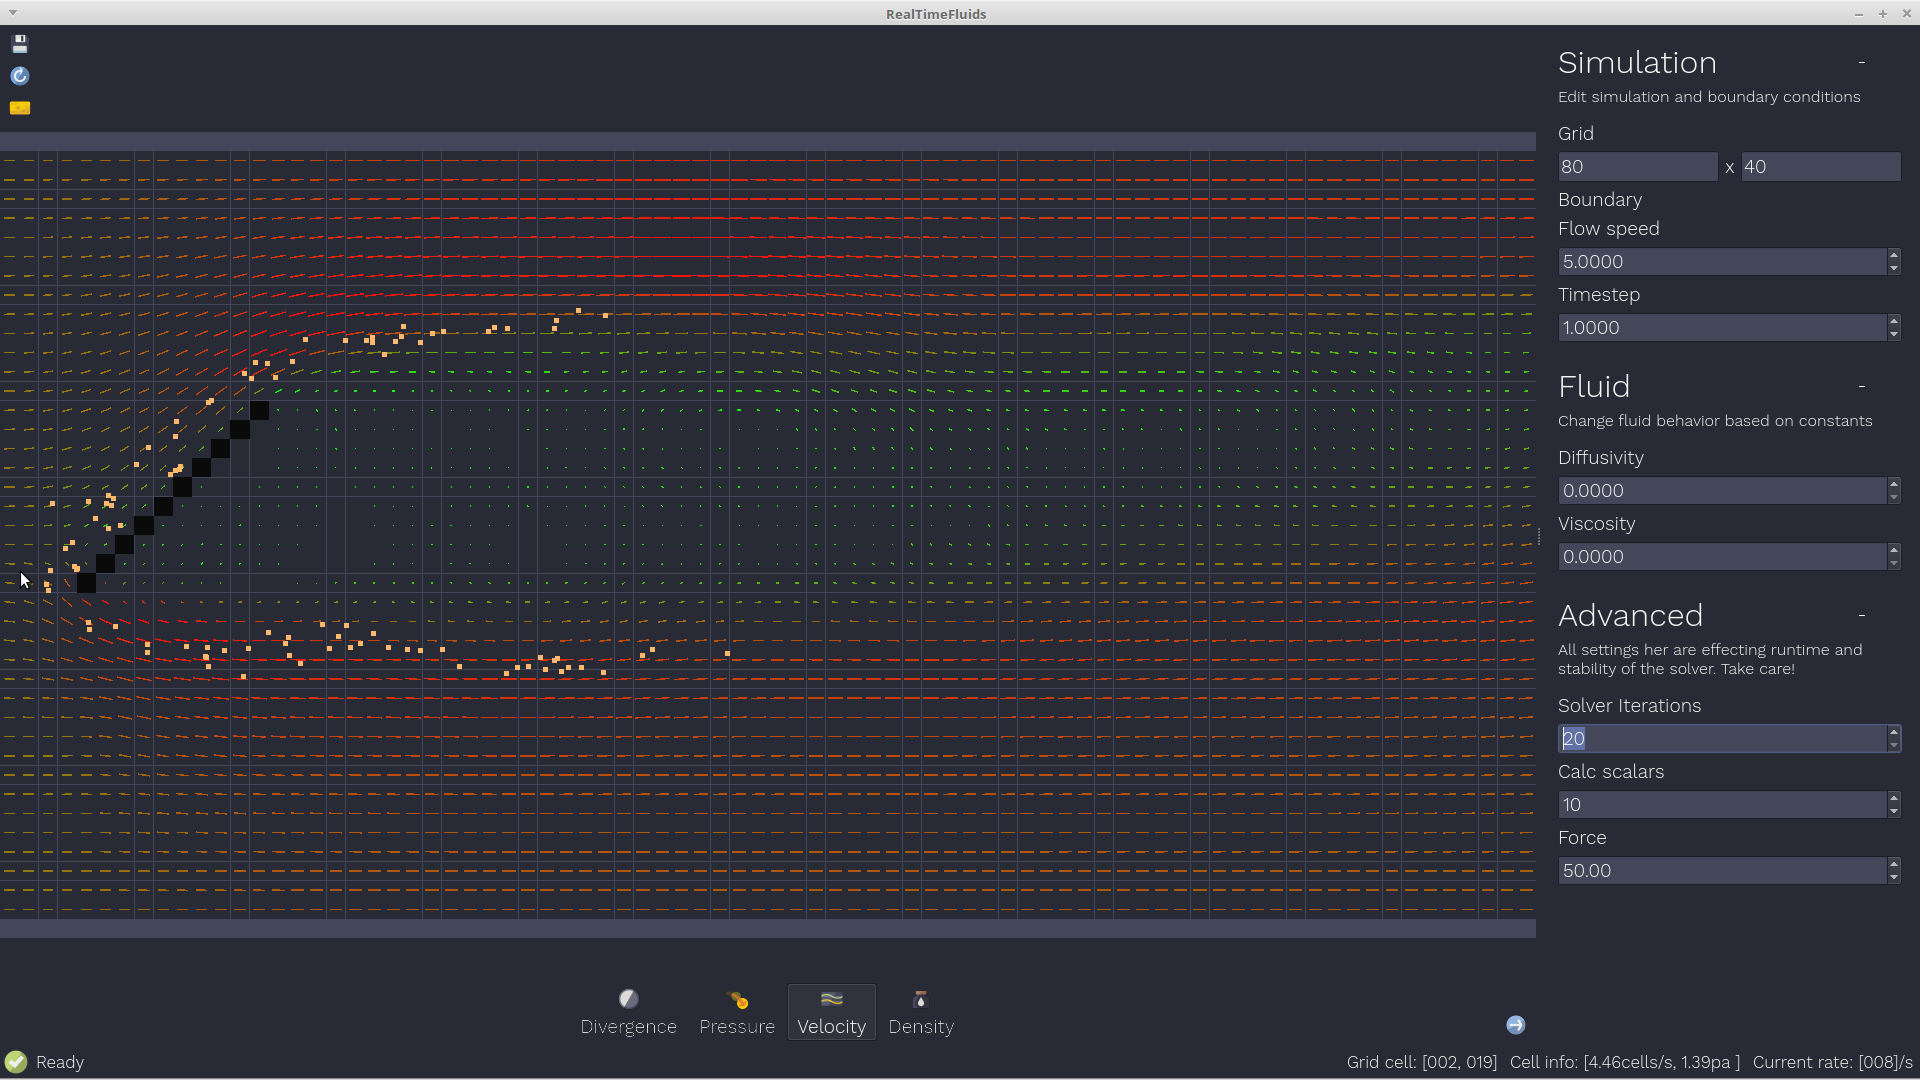
\includegraphics[width=\textwidth]{images/Particle.png}
	\caption{Einfache Partikel}
	\label{fig:Partikel}
\end{figure}

In allen vier Ansichten ist es m\"oglich, mit der \textit{linken Maustaste} Partikel hinzuzuf\"ugen. Diese werden beim \"Andern der Ansicht auch weiterhin angezeigt. Falls der Benutzer mehrere Partikel setzen will, kann er beim Bewegen der Maus \"uber das Str\"omungsfeld die linke Maustaste gedr\"uckt halten.

Um externe Kr\"afte innerhalb des Str\"omungskanals aufzubringen, muss der Benutzer die Tastenkombination \textit{Control halten + linke Maustaste} benutzen. Nach dem Halten der Control Taste dr\"uckt der Benutzer an die gew\"unschte Stelle im Kanal (um den Ausgangspunkt der Kraft auszuw\"ahlen), h\"alt dabei die Maustaste gedr\"uckt und bewegt den Zeiger in eine beliebige Richtung. Sobald er dann die Maustaste losl\"asst, wird die Kraft, ausgehend vom Ausgangspunkt, in die vorgegebene Richtung aufgebracht. Um die Kraft erneut an der gleichen Stelle aufzubringen, kann der Benutzer im Anschluss die Kombination aus \textit{Control halten + rechte Maustaste}, mit dem gleichen Vorgehen, benutzen. Dabei ist es egal, an welcher Position innerhalb des Str\"omungskanals die Kraft mit dem Zeiger aufgebracht wird. Eine externe Kraft kann nur aufgebracht werden, wenn eine Richtung vorgegeben wird. Die externen Kr\"afte sind in Form einer Geschwindigkeit, die man in das Feld aufbringt.

F\"ur das Setzen von Hindernissen an der vom Mauszeiger ausgew\"ahlten Stelle muss der Benutzer die Tastenkombination \textit{Shift halten + linke Maustaste} benutzen. Ein Hindernis f\"ullt jeweils die gesamte Zelle des Str\"omungskanals aus. Um ein Hindernis an der vom Mauszeiger ausgew\"ahlten Stelle wieder zu l\"oschen, benutzt er \textit{Shift halten + rechte Maustaste}. Falls der Benutzer mehrere Hindernisse l\"oschen oder setzen will, kann er die linke beziehungsweise rechte Maustaste gedr\"uckt halten und anschlie\ss end \"uber die gew\"unschten Positionen ziehen.

\item[In der Geschwindigkeitsfeld Ansicht:] ~

\begin{figure}[H]
	\centering
	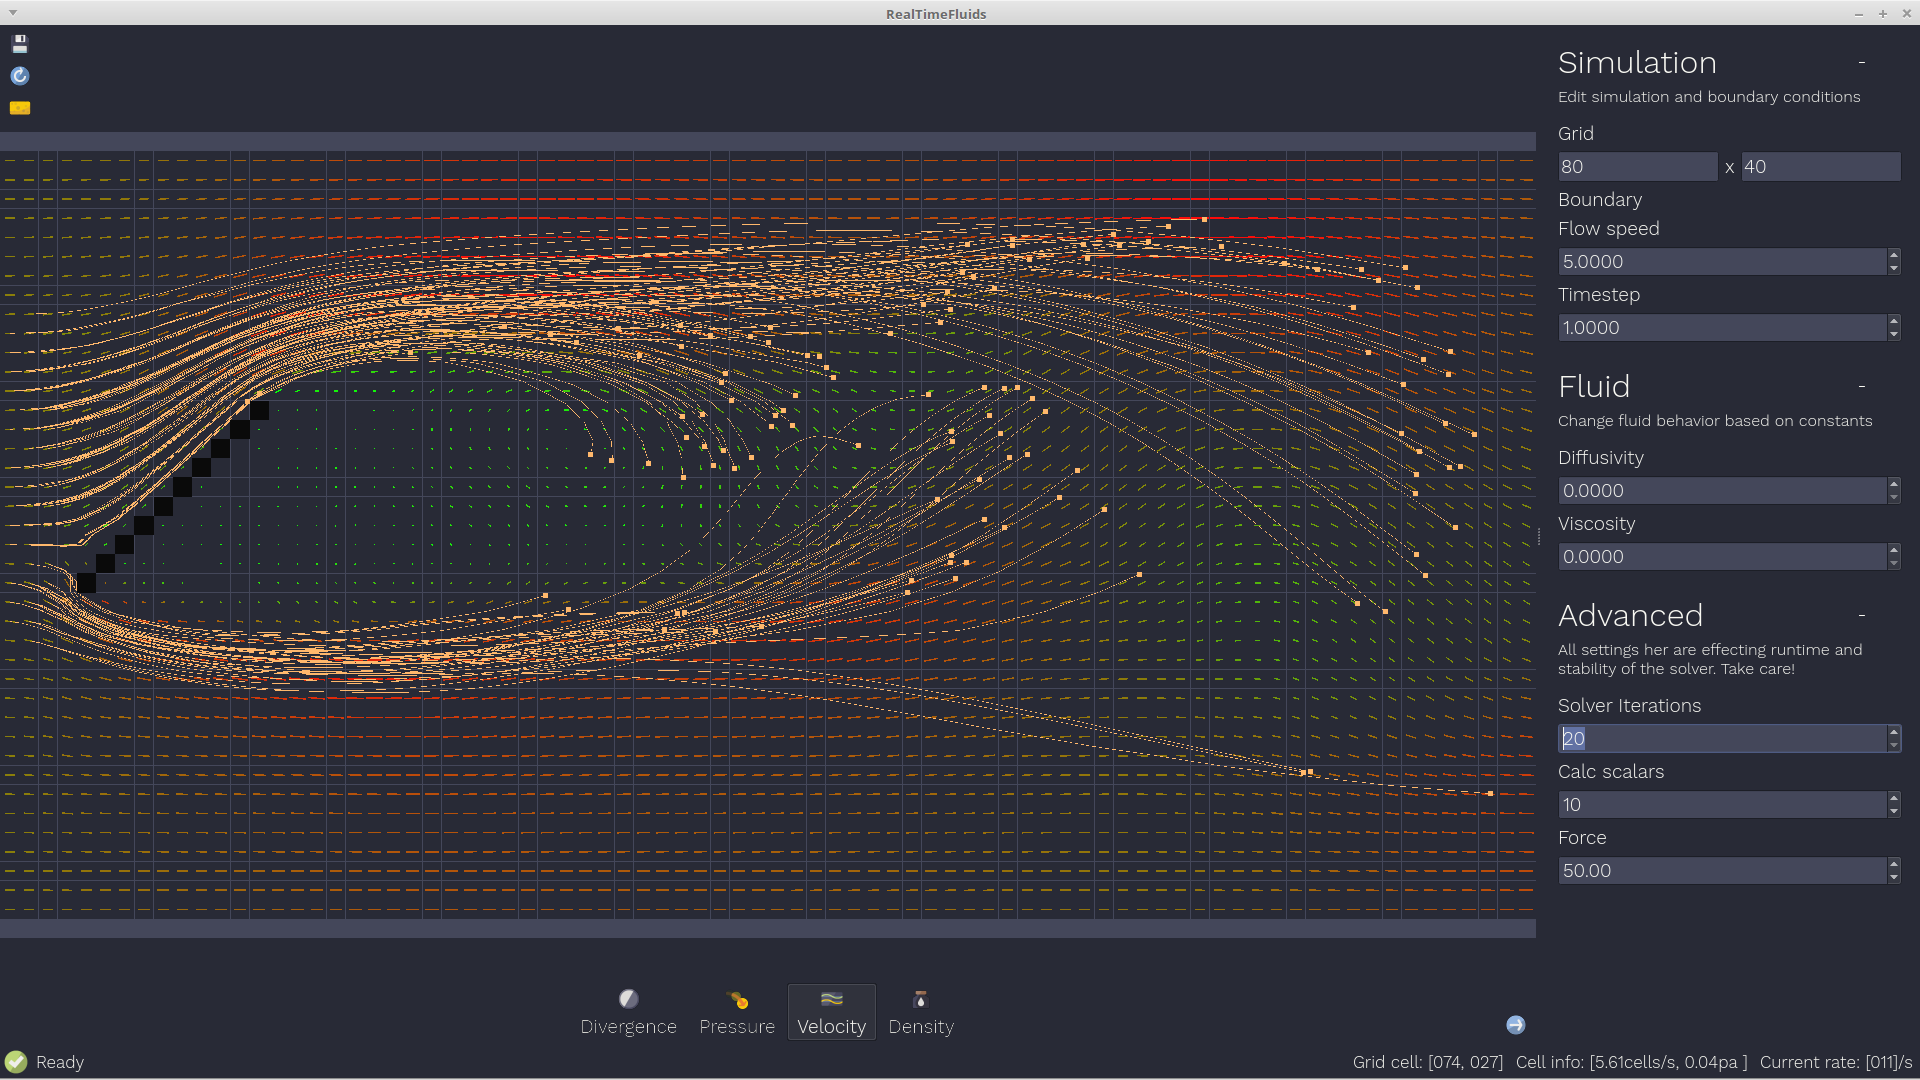
\includegraphics[width=\textwidth]{images/Particle_Trajectory.png}
	\caption{Partikel mit Bahnlinie}
	\label{fig:Partikel_Bahnlinie}
\end{figure}

Eine Interaktion, die nur im Geschwindigkeitsfeld m\"oglich ist, ist das Hinzuf\"ugen von Partikeln mit Bahnlinien. Um ein Partikel hinzuzuf\"ugen, dessen Bahnlinie im Str\"omungsfeld eingezeichnet wird, wird die \textit{rechte Maustaste} benutzt. Falls der Benutzer mehrere Partikel setzen will, kann er beim Bewegen der Maus \"uber das Str\"omungsfeld die rechte Maustaste gedr\"uckt halten. Partikel mit Bahnlinien werden jeweils nur in den Zellmittelpunkten erzeugt.
Obwohl das hinzuf\"ugen dieser Partikel nur in der Ansicht des Geschwindigkeitsfeldes m\"oglich ist, werden die Bahnlinien trotzdem in allen Ansichten angezeigt.

\item[In der Dichteverteilungsfeld Ansicht:] ~

Mit der \textit{rechten Maustaste} kann im Dichteverteilungsfeld Tinte hinzugef\"ugt werden. Falls der Benutzer kontinuierlich Tinte hinzuf\"ugen will, kann er die rechte Maustaste gedr\"uckt halten, w\"ahrend er  die Maus \"uber das Str\"omungsfeld zieht. Das Hinzuf\"ugen von Tinte dient zur Veranschaulichung von Dichteverteilungen innerhalb des Str\"omungsfeldes. Dabei ist zu beachten, dass vor allem bei hohen Einflussgeschwindigkeiten, diese Verteilung sehr schnell verlaufen kann. Zur Demonstration sollten deshalb der \textit{Flow speed} und die \textit{Diffusivity} niedrig sein.

\end{description}
F\"ur ein schnelles L\"oschen aller Hindernisse oder das Entfernen von Partikeln, siehe \hyperref[sec:neuundzurueck]{\textcolor{blue}{Simulation Neu Starten und Zur\"ucksetzen}}

\subsection{Sidebar}

Auf der rechten Seite, der sogenannten Sidebar, kann der Benutzer die Randbedingung und Simulationswerte eingeben. Die jeweiligen G\"ultigkeitsbereiche dieser Werte sind im Anschluss zu finden.

\begin{figure}[H]
	\centering
	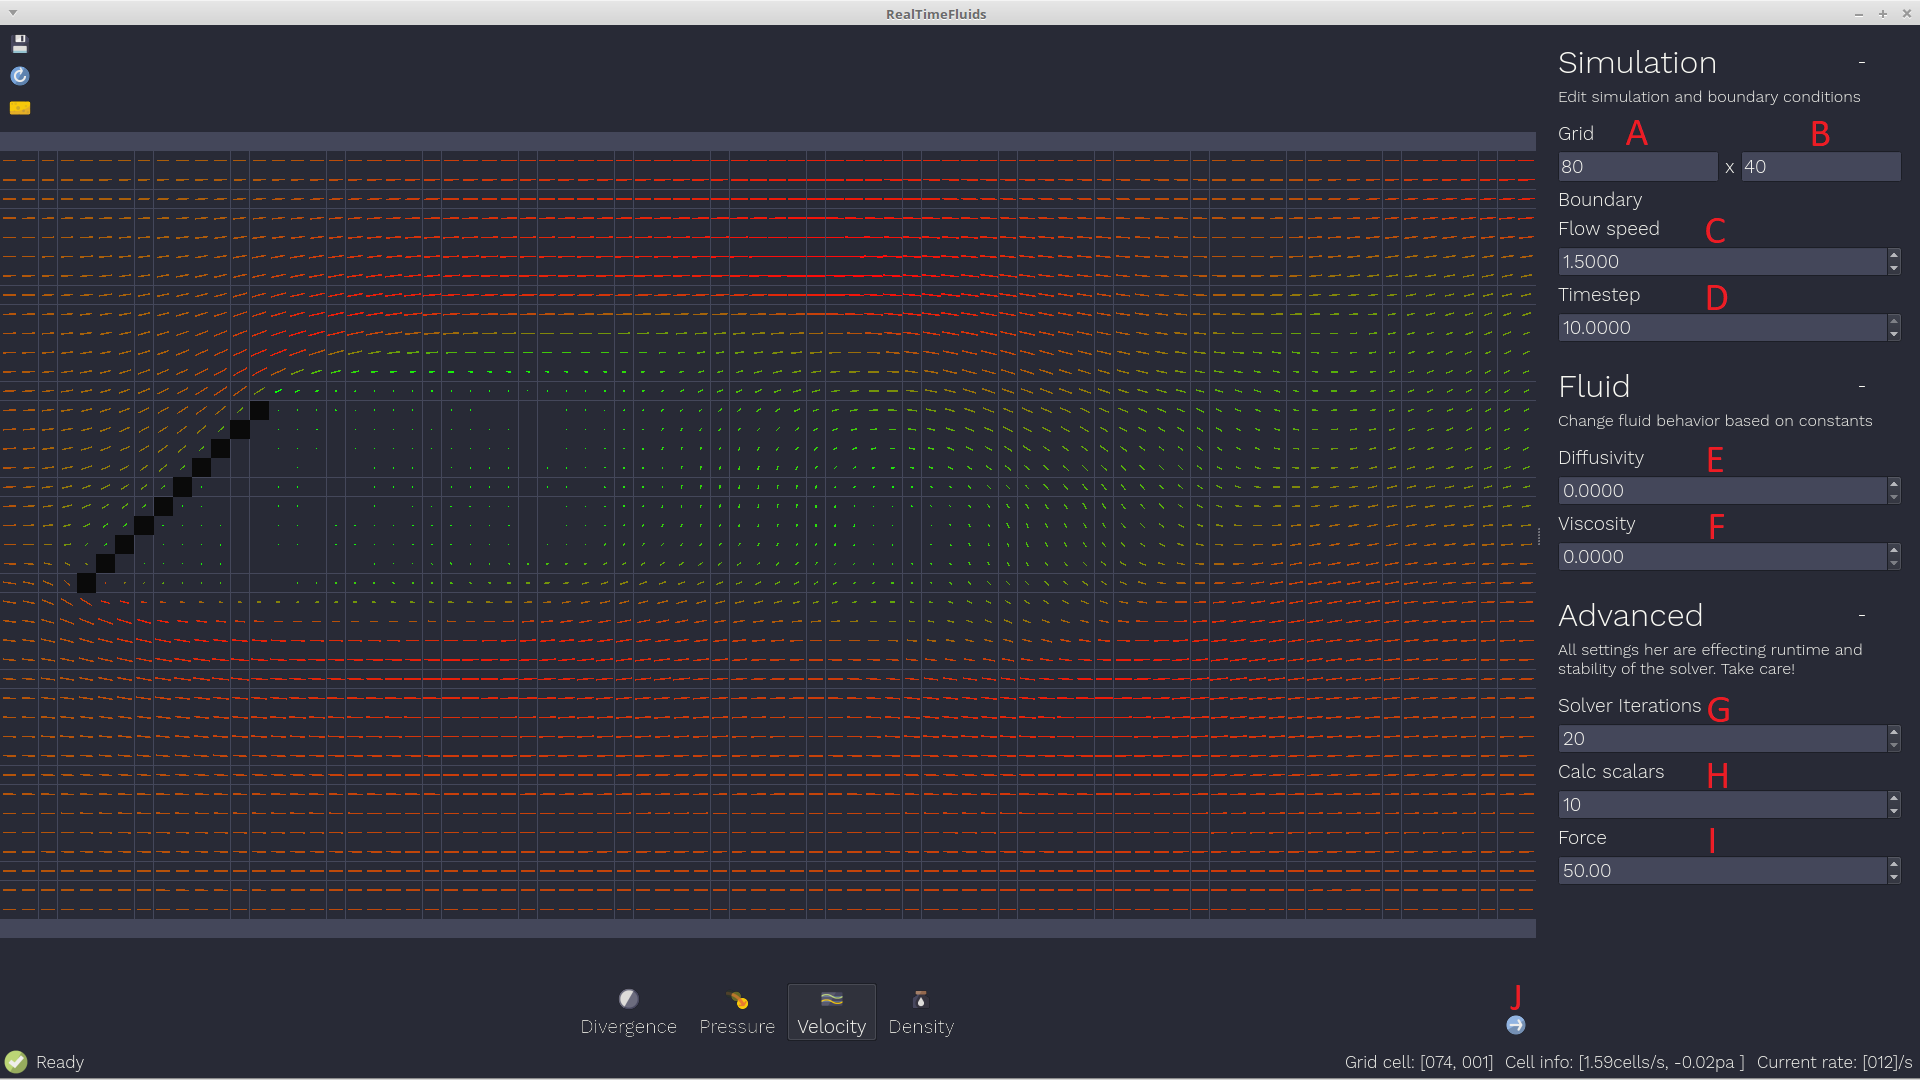
\includegraphics[width=\textwidth]{images/Sidebar.png}
	\caption{Sidebar}
	\label{fig:Sidebar}
\end{figure}

\begin{itemize}

\item \textit{Feld A} beinhaltet die Anzahl der Zellen in der Breite des Str\"omungskanals.
\item \textit{Feld B} beinhaltet die Anzahl der Zellen in der H\"ohe des Str\"omungskanals.

Die Dimension des Str\"omungskanals ist nur nach unten gekappt, es kann also beliebig gro\ss{}  gew\"ahlt werden. Hier ist Vorsicht geboten, da bei hoher Anzahl die Rechnerleistung meistens nicht mehr ausreicht. F\"ur normale Rechner ist ein Maximum von 1000 zu empfehlen.
\item \textit{Feld C} ist die Einflussgeschwindigkeit des Fluids am linken Rand des Str\"omungskanals. Sie hat die Einheit Zelle pro Sekunde.
\item \textit{Feld D} ist der Zeitschritt der Simulation. Er bestimmt das Verh\"altnis zwischen Echt- und Simulationszeit.
\item \textit{Feld E} ist der Diffusionskoeffizient. Er bestimmt die Beweglichkeit der Tintefluidteilchen.
\item \textit{Feld F} ist die Viskosit\"at. Sie bestimmt die Z\"ahfl\"ussigkeit des Fluids.
\item \textit{Feld G} ist die Anzahl der Iterationen des numerischen L\"osungsverfahren. Je h\"oher der Wert, desto genauer wird die Simulation.
\item \textit{Feld H} ist die Rate der Skalar Berechnung. Genauer gesagt, wie oft sich das Farbfeld der Str\"omung und die Werte auf der Statusbar aktualisieren.
\item \textit{Feld I} ist die Gr\"o\ss e der externen Kraft, die im Str\"omungsfeld eingebracht werden kann. Sie hat die Einheit $\frac{cells}{s}$.
\item \textit{Feld J} dient zum Aus- und Einblenden der Sidebar. Dabei wird das Bild des Str\"omungsfeldes vergr\"o\ss ert beziehungsweise verkleinert.

\end{itemize}
Die einzelnen Felder haben folgende Grenzen beziehungsweise G\"ultigkeitsbereiche:
\begin{itemize}
\item Gittergr\"o\ss e (Reihen sowie Spalten): 10-unbegrenzt (Hinweis siehe oben)
\item Einflussgeschwindigkeit: 0 - 10 $\frac{cells}{s}$
\item Zeitschritt: 0.0001 - 10
\item Diffusionskoeffizient: 0 - 100
\item Viskosit\"at: 0 - 1000
\item L\"oseriterationen: 20 - 5000
\item Rate der Skalar Berechnung: 1 - 1000
\item Externe Kraft: 0 - 100 $\frac{cells}{s}$
\end{itemize}

\textit{Sidebar Abschnitte ausblenden:}

\begin{figure}[H]
	\centering
	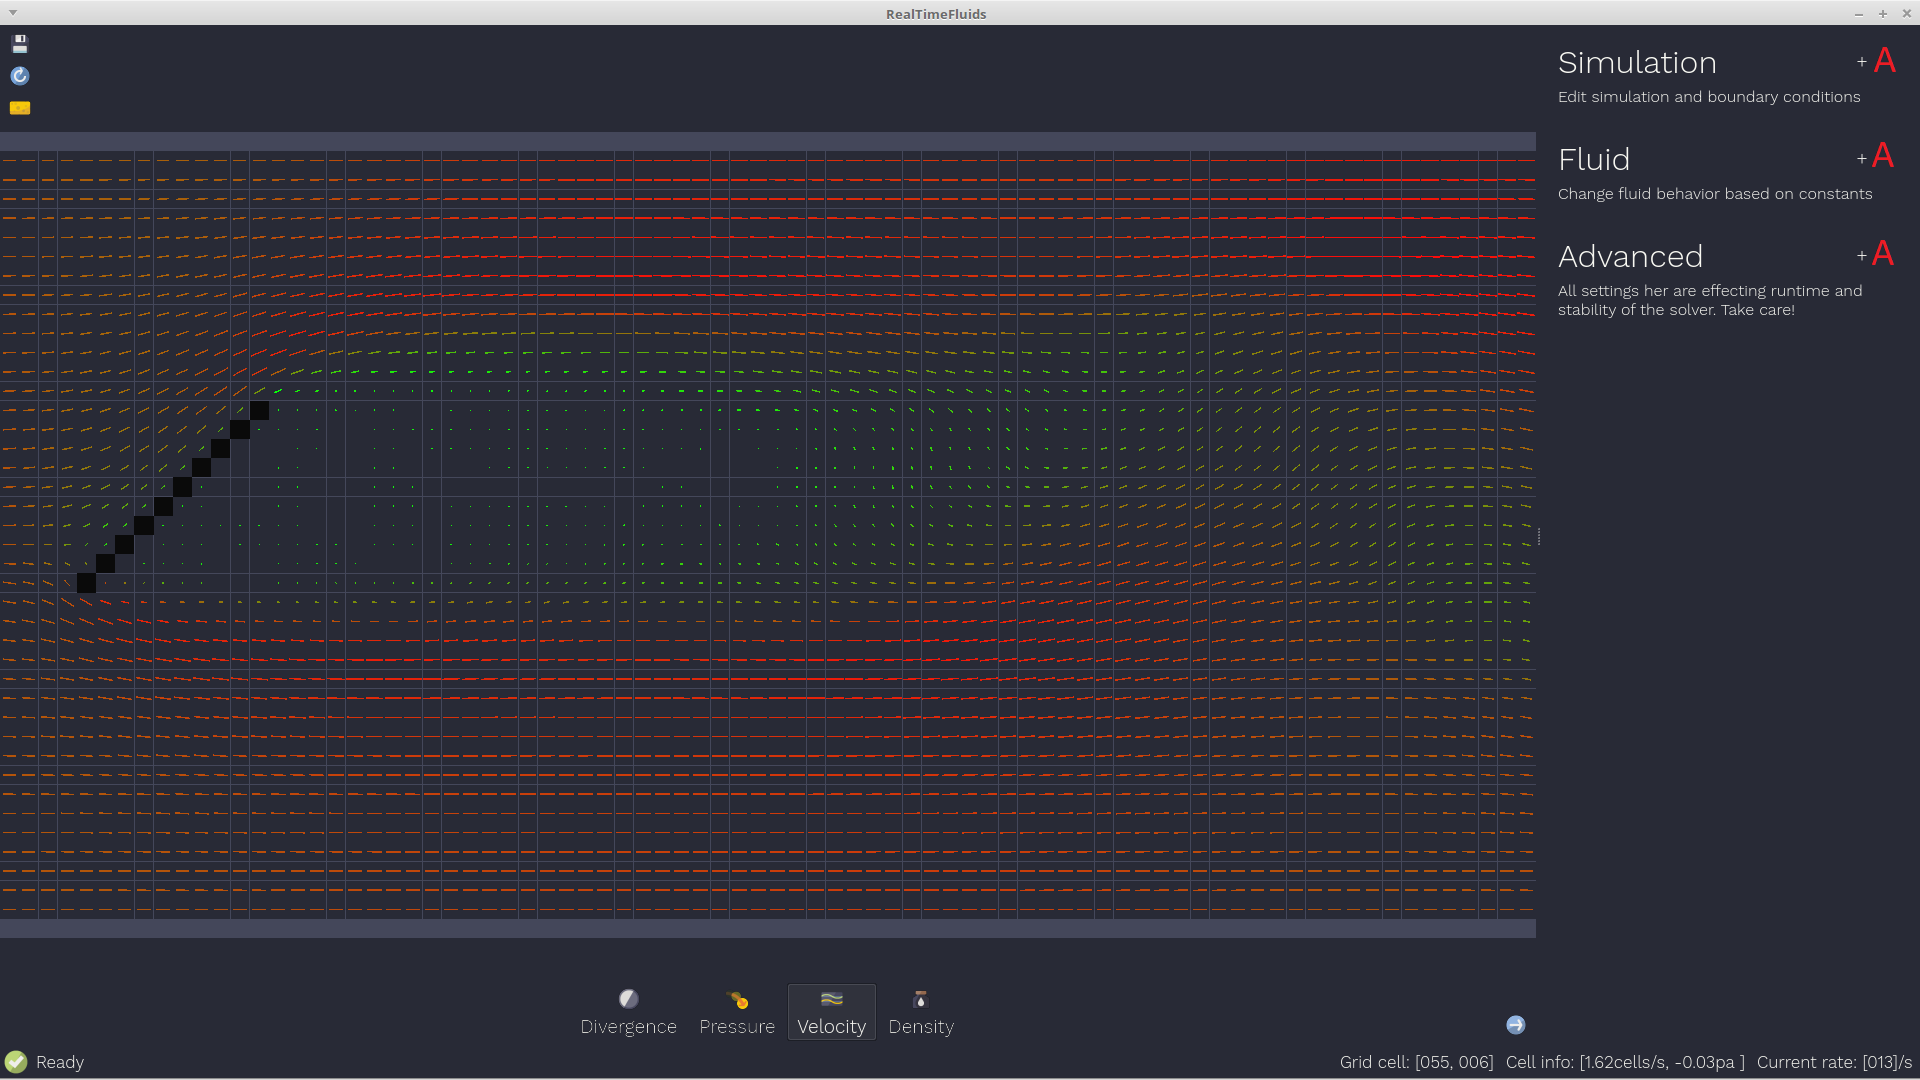
\includegraphics[width=\textwidth]{images/Input_Collapsed.png}
	\caption{Abschnitte ausgeblendet}
	\label{fig:Abschnitte_ausgeblendet}
\end{figure}

Wenn der Benutzer die Simulationswerte nicht weiter ver\"arendern will, kann er in den \textit{Feldern A} die jeweiligen Abschnitte minimieren (""-"" Symbol) und im Anschluss wieder aufrufen (""+"" Symbol).

\subsection{Statusbar}
\begin{figure}[H]
	\centering
	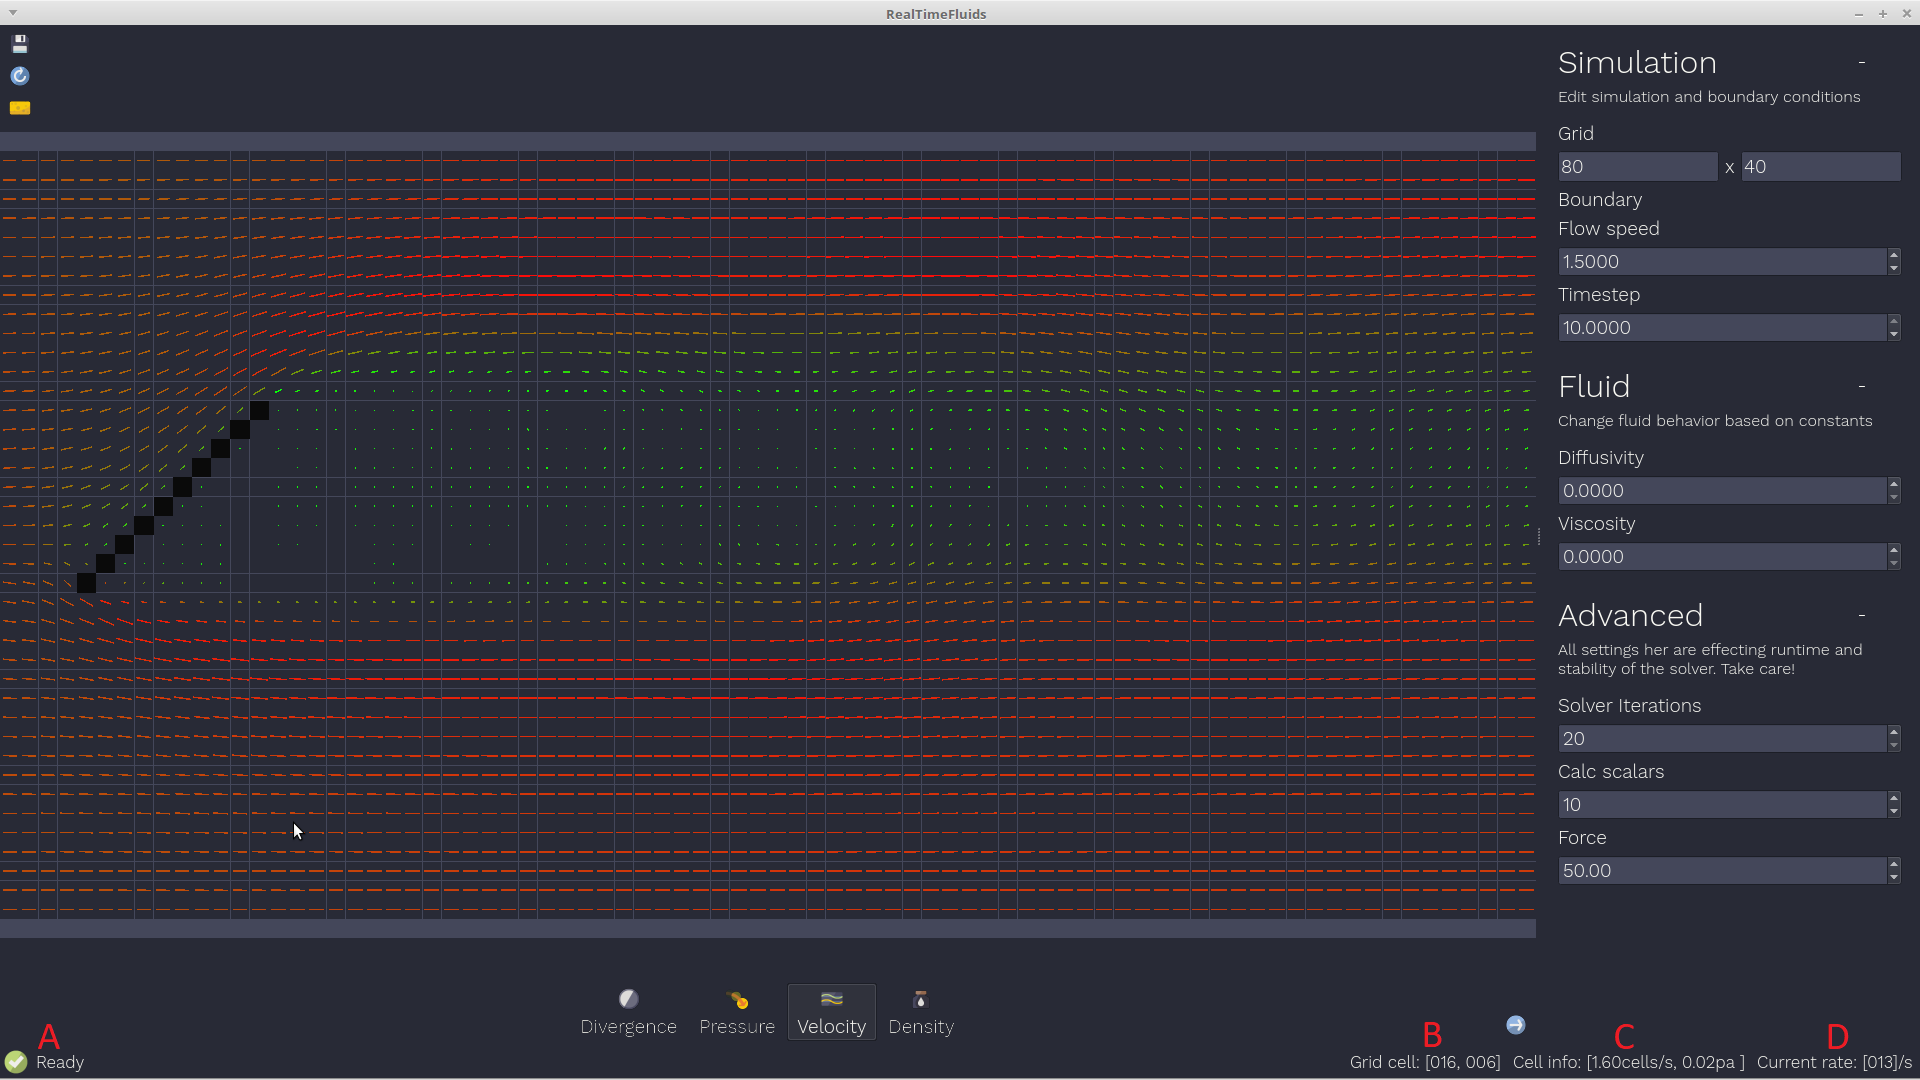
\includegraphics[width=\textwidth]{images/Statusbar.png}
	\caption{Statusbar}
	\label{fig:Statusbar}
\end{figure}

\begin{itemize}

\item \textit{Feld A} zeigt den Stand der Simulation an. Hier erscheinen potentielle Fehlermeldungen.
\item \textit{Feld B} zeigt die Position des Mauszeigers innerhalb des Str\"omungsfeldes. Das Format ist [Breite,H\"ohe].
\item \textit{Feld C} zeigt die aktuelle Geschwindigkeit in $\frac{cells}{s}$ und den Druck in [Pa] des Feldes, auf dem sich der Mauszeiger befindet.
\item \textit{Feld D} zeigt die aktuelle $\frac{Aktualisierungsrate}{s}$ des Str\"omungsfeldes. Sie ist vor allem von der Anzahl der numerischen L\"oseriterationen abh\"angig und passt sich adaptiv an.

\end{itemize}

\subsection{Simulation Laden und Speichern}

\begin{figure}[H]
	\centering
	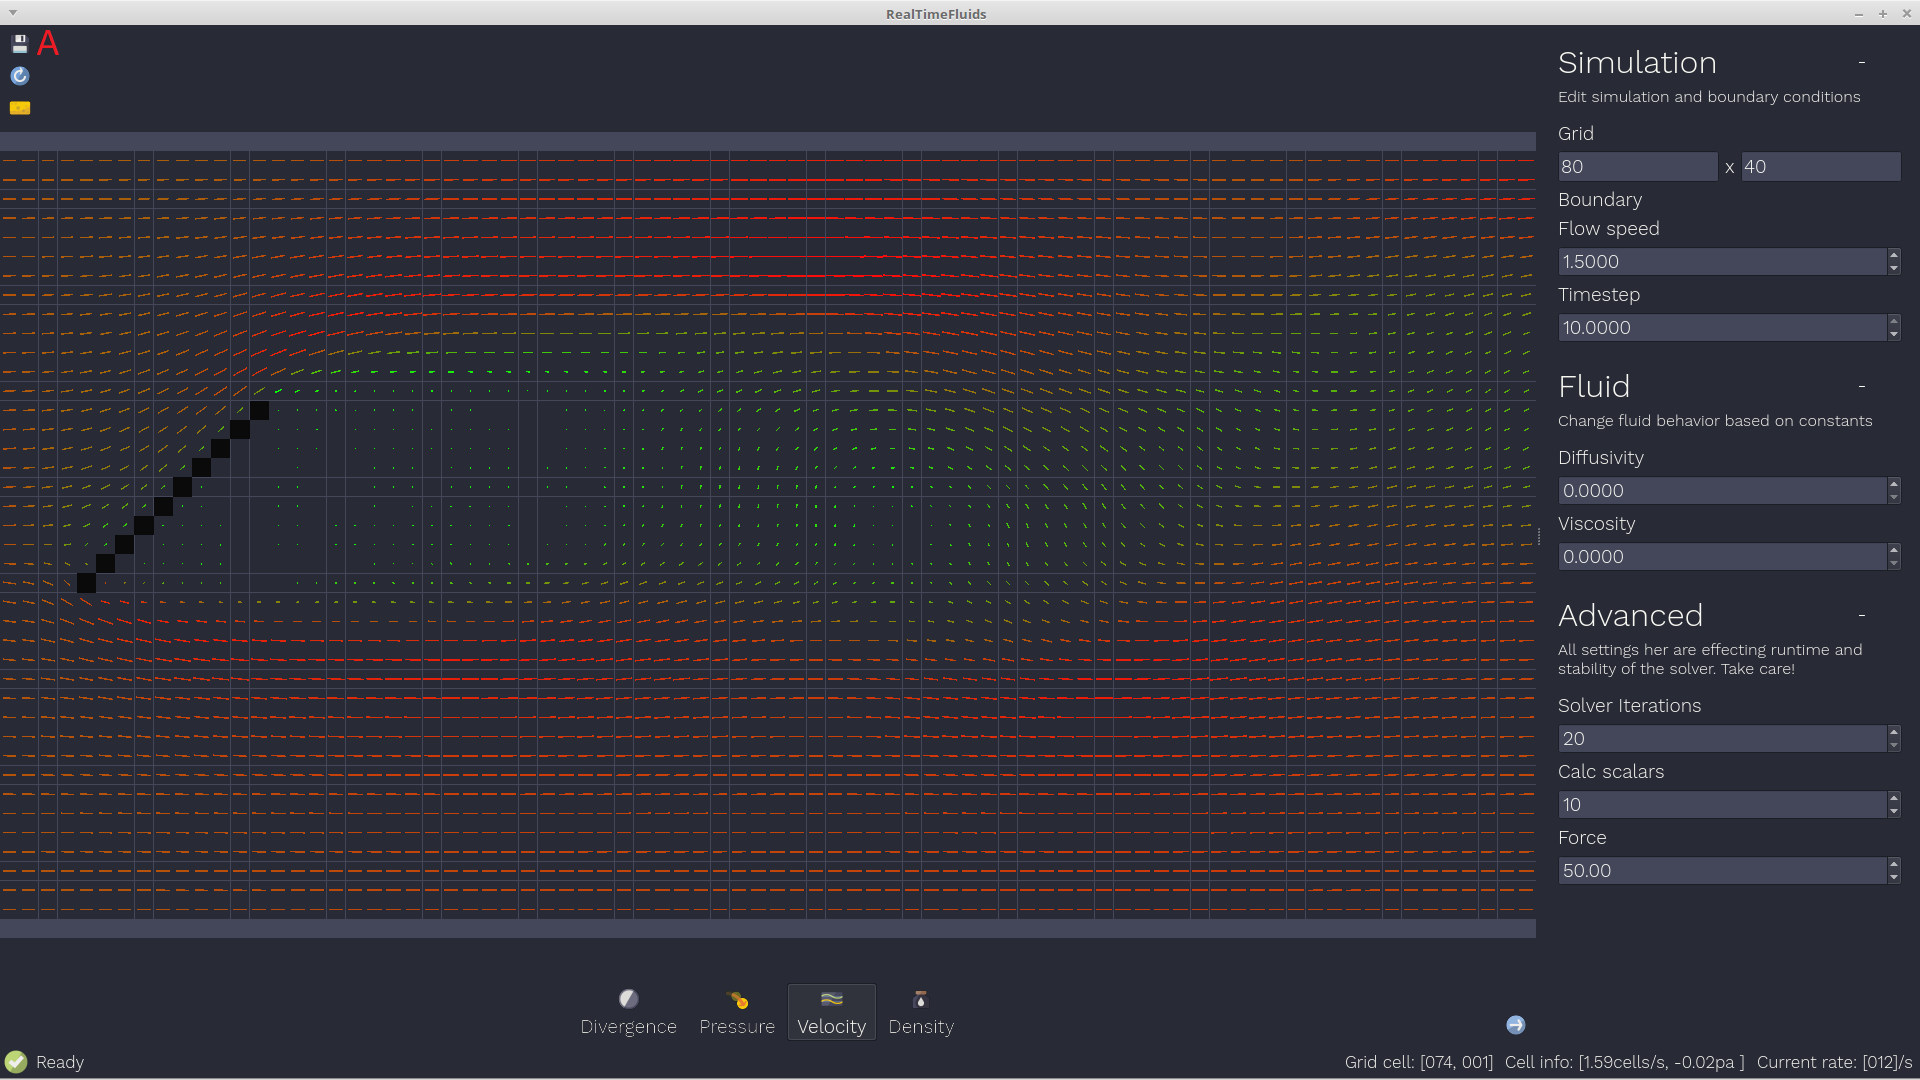
\includegraphics[width=\textwidth]{images/Select_Load.png}
	\caption{Simulation Laden und Speichern Men\"u}
	\label{fig:sim_lad_speich_men}
\end{figure}

\"Uber das \textit{Feld A} gelangt man in das Men\"u zum Laden und Speichern von Simulationen:

\begin{figure}[H]
	\centering
	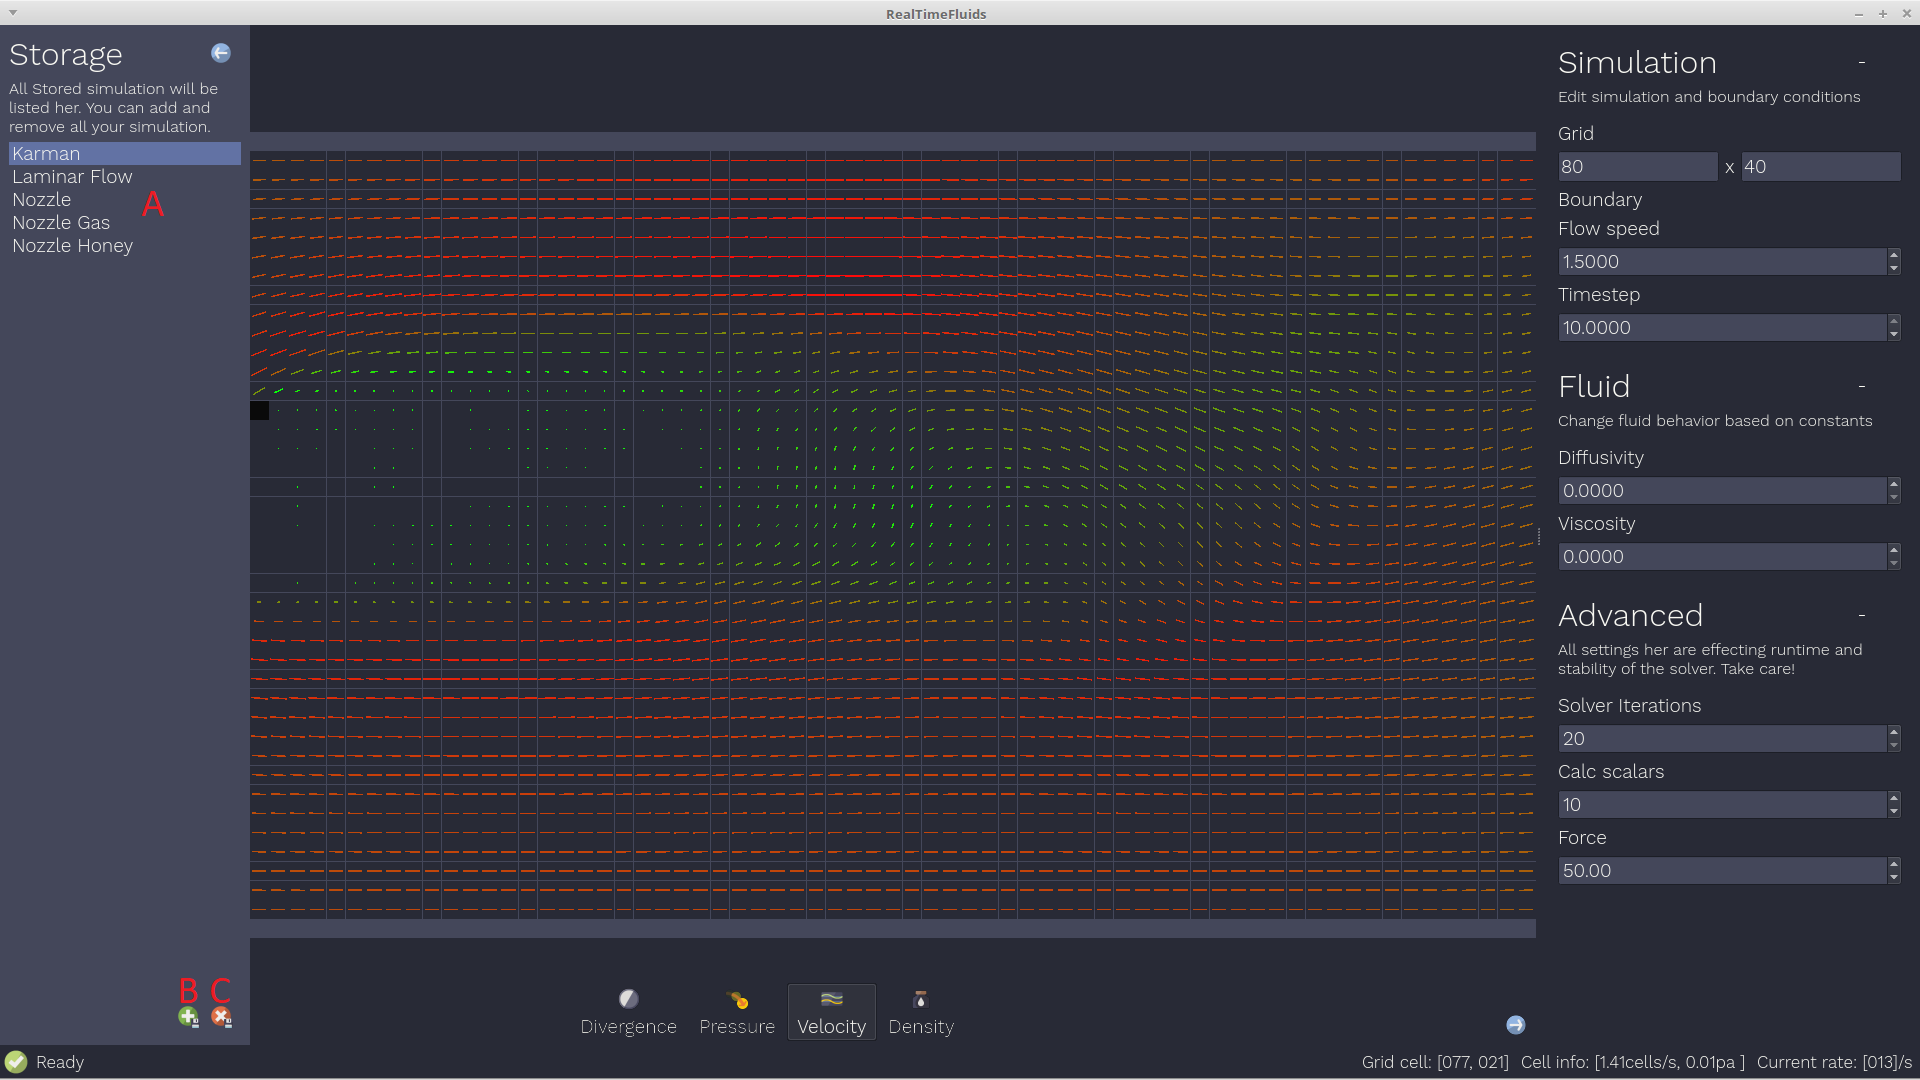
\includegraphics[width=\textwidth]{images/Load_Simulation.png}
	\caption{Simulation Laden und Speichern}
	\label{fig:sim_lad_speich}
\end{figure}

Das \textit{Feld A} zeigt alle aktuell gespeicherten Simulationen. Um eine gew\"unschte Simulation aus dieser Liste zu laden, muss man sie mit der linken Maustaste ausw\"ahlen. Um eine bereits existierende Simulation umzubenennen, klickt der Benutzer doppelt mit der linken Maustaste direkt auf den Namen der Simulation. Mehrere gleich benannte Simulationen darf es dabei nicht geben.

Das Programm \"uberschreibt die aktuelle Simulation automatisch, sobald man einen Wert (au\ss er der Gittergr\"o\ss e) \"andert. Die Gittergr\"o\ss e wird gespeichert, sobald man die Simulation neu startet oder das Simulationsprogramm schlie\ss t.

Um Platz zum Speichern einer weiteren Simulation zu machen, dr\"uckt der Benutzer auf das \textit{Feld B}.

Um eine in der Liste existierende Simulation zu l\"oschen, w\"ahlt man die gew\"unschte Simulation per Mausklick aus und dr\"uckt auf das \textit{Feld C}.


\subsection{Simulation Neu Starten und Zur\"ucksetzen}
\label{sec:neuundzurueck}

\begin{figure}[H]
	\centering
	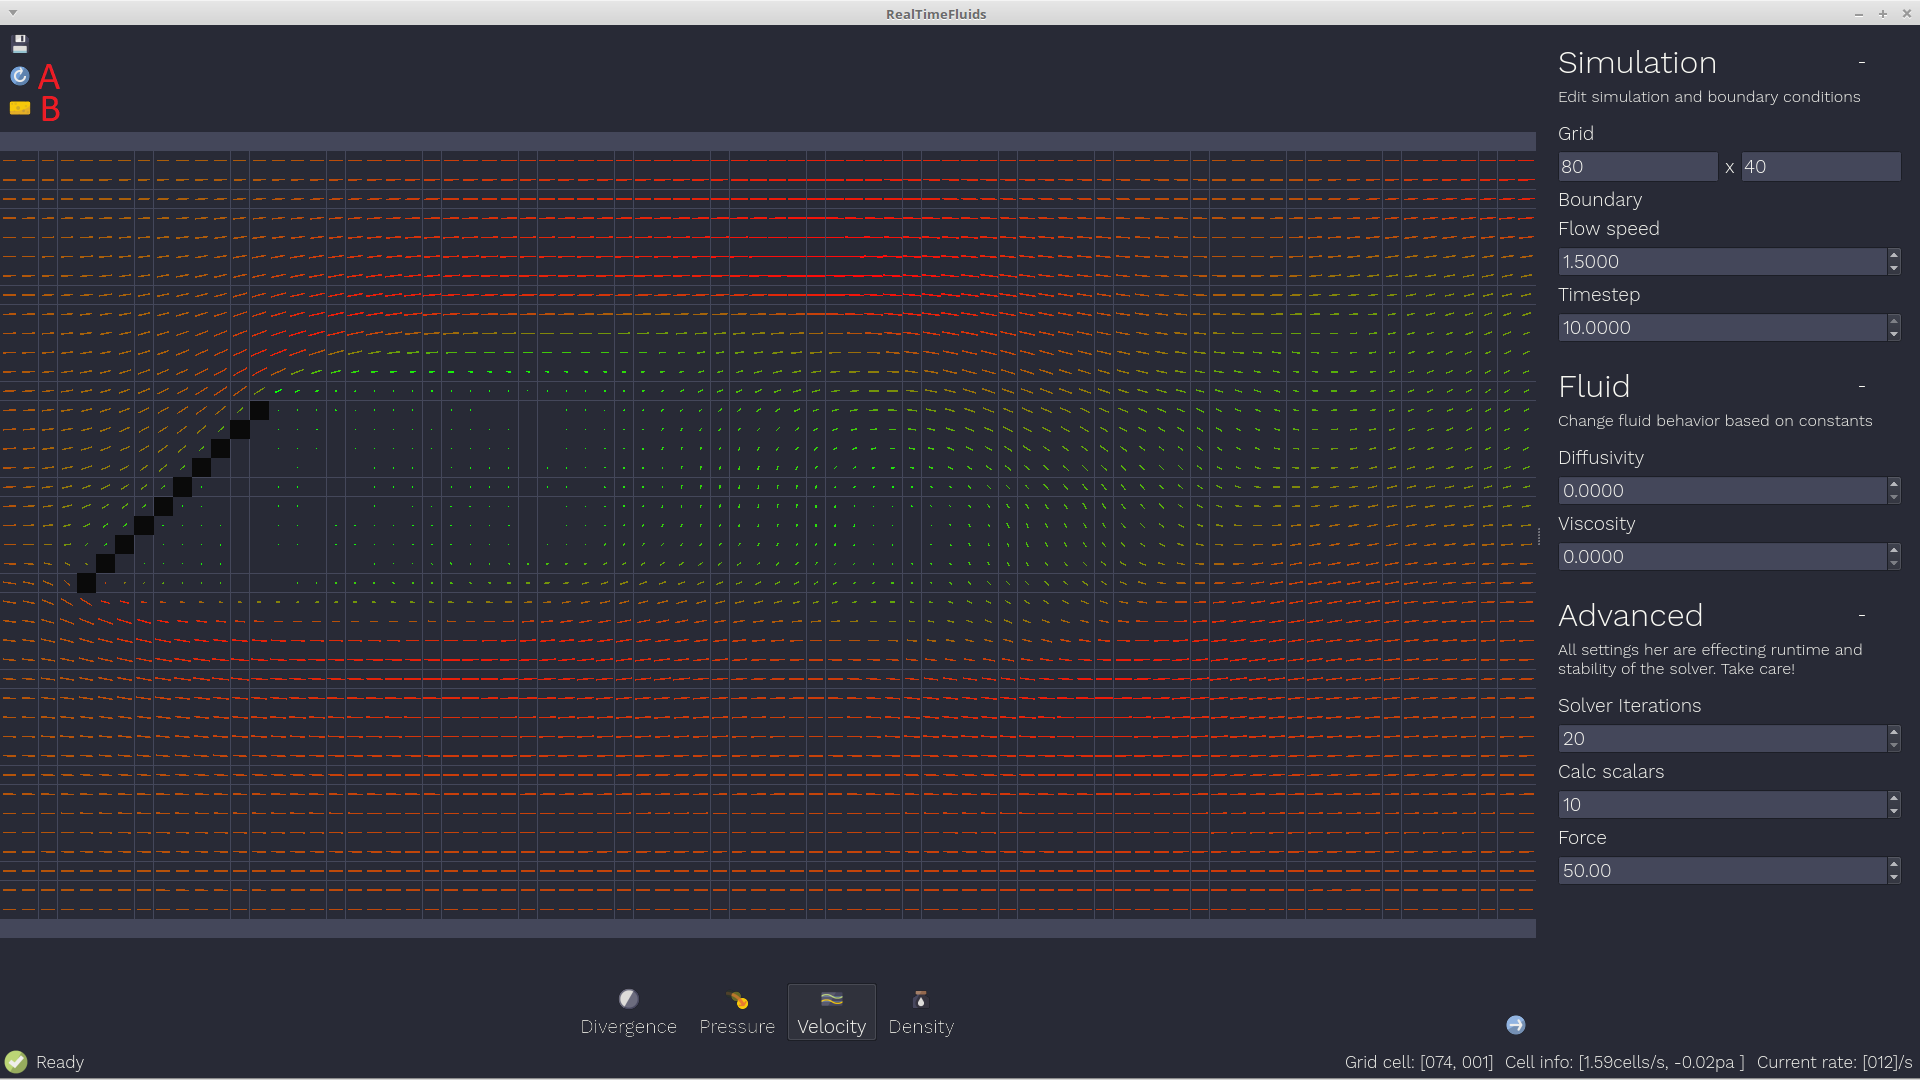
\includegraphics[width=\textwidth]{images/Clear_Restart.png}
	\caption{Simulation neu Starten oder Zur\"ucksetzen}
	\label{fig:sim_neu_zurueck}
\end{figure}

Das \textit{Feld A} startet die Simulation neu. Dabei wird auch, falls ge\"andert, die Gittergr\"o\ss e angepasst. Es bedeutet, dass alle Hindernisse, Partikel und Bahnlinien im Str\"omungsfeld gel\"oscht werden.   

Das \textit{Feld B} setzt die Simulation zur\"uck. Die Hindernisse bleiben erhalten, die Gittergr\"o\ss e bleibt unver\"andert. Das einzige was gel\"oscht wird, sind die Partikel samt Bahnlinien.

\section{Fehlersituationen}

Bei der Benutzung dieser Simulationssoftware sind zwei Fehlermeldungen, die jeweils in der Statusbar bei \textit{Feld A} zu sehen sind, m\"oglich.
\begin{figure}[H]
	\centering
	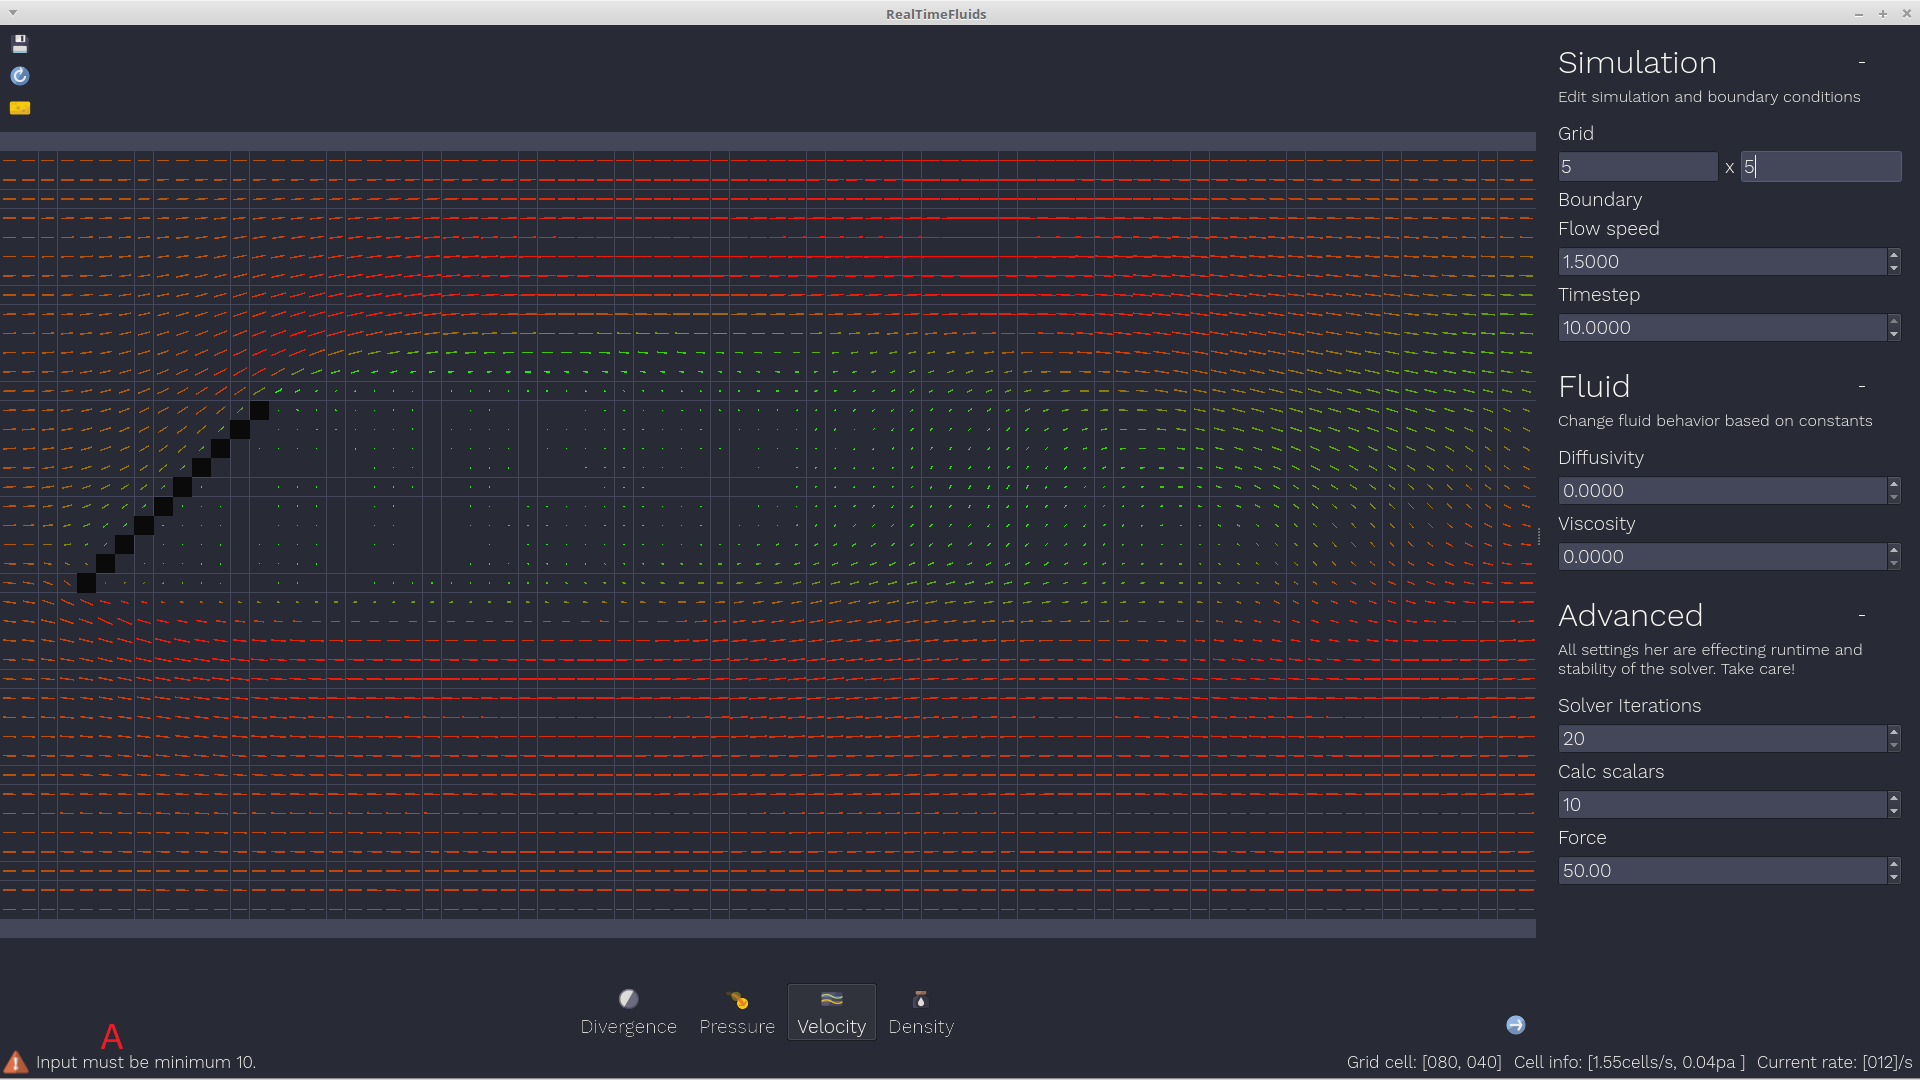
\includegraphics[width=\textwidth]{images/Gridsize_Error.png}
	\caption{Fehler bei Gittergr\"o\ss enwahl}
	\label{fig:Fehler_Gitter}
\end{figure}

Die erste Fehlermeldung, "'Input must be minimum 10."', erscheint, falls der Benutzer eine Gittergr\"o\ss e kleiner 10 w\"ahlen will. Dies gilt f\"ur die Breite sowie H\"ohe des Str\"omungsfeldes. Die Fehlermeldung verschwindet, sobald der Benutzer einen Wert gr\"o\ss er gleich 10 w\"ahlt, oder nach einigen Sekunden automatisch. Die Simulationsaktualisierung kann erst erfolgen, wenn ein Wert gr\"o\ss er gleich 10 gew\"ahlt wurde. Falls der Benutzer die Simulation mit einem ung\"ultigen Wert neu startet, wird automatisch mit dem g\"ultigen vorherigen Wert \"uberschrieben.

\begin{figure}[H]
	\centering
	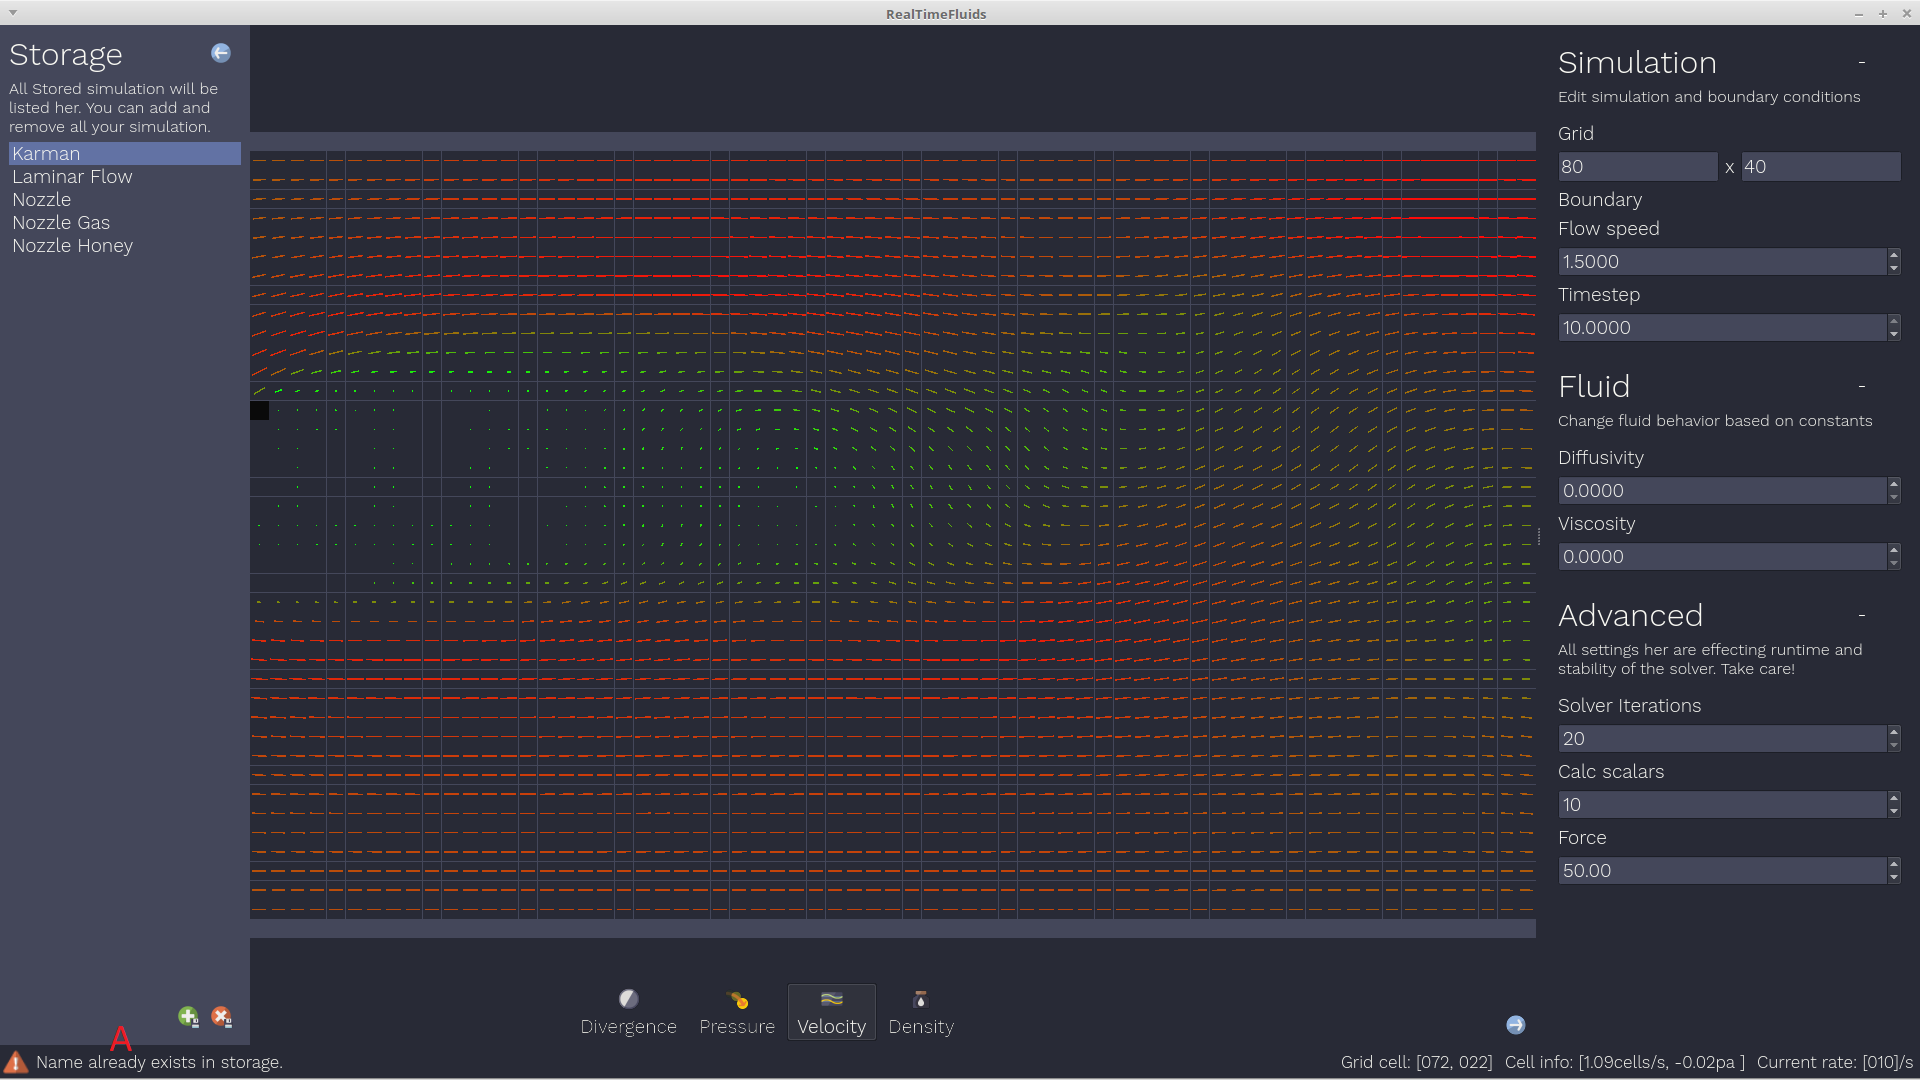
\includegraphics[width=\textwidth]{images/Name_Duplicate.png}
	\caption{Namenskonflikt}
	\label{fig:Namenskonflikt}
\end{figure}

Die zweite Fehlermeldung, "'Name already exists in storage."', erscheint, falls der Benutzer eine Simulation umbenennen will aber bereits eine Simulation unter diesem Namen gespeichert ist. Falls der Benutzer trotzdem den ung\"ultigen Namen best\"atigen will, wird automatisch mit dem vorherigen g\"ultigen Namen \"uberschrieben.

\chapter{Entwicklerdokumentation}

Im Gegensatz zu einer Benutzerdokumentation ist diese Dokumentation sehr detailliert und geht direkt auf den Quellcode ein.

\section{Codestruktur}

Die Codestruktur ist dem Klassendiagramm (siehe \hyperref[sec:Klassenkapitel]{\textcolor{blue}{Klassendiagramme}}) zu entnehmen. Detaillierte Informationen \"uber eine Klasse sind Doxygen zu entnehmen (siehe \hyperref[sec:doxygenerzeugung]{\textcolor{blue}{Doxygen}}).

\section{Detailierte Dokumentation des Codes}
\label{sec:doxygenerzeugung}

Doxygen kann aus der Konsole erzeugt werden. Navigieren Sie hierf\"ur zuerst in den Ordner \textit{code}. F\"uhren Sie danach den Befehl  \textit{doxygen Doxyfile} in der Konsole aus. Die Dokumentation befindet sich dann im Ordner \textit{doc/doxygen}.

\section{Software Tests}

Die Simulation wurde auf Windows 10 (MinGW GNU 5.4 und QT 5.8), Ubuntu 16.04 (GNU 5.4 und QT 5.5), dem RWTH High-Performance Cluster (clang 4.0.1 und QT 5.9.1) und MacOS Sierra 10.12.6 (GNU 6.4 und QT 5.9.1) erfolgreich compiliert und getestet.

\bibliographystyle{plain}
\bibliography{literatur}

\appendix

F\"ur der Entwicklung dieser Software bezogen wir uns vor allem auf folgende Literaturen:

\begin{enumerate}
  \item Stable Fluids by Jos Stam (1999)
  \item Real-Time Simulation and Rendering of 3D Fluids by Crane et al. (2007)
  \item Real-Time Fluid Dynamics for Games by Jos Stam (2003)
\end{enumerate}

\chapter{Quellcode}

Der Quellcode unserer Software ist im Ordner code/src zu finden.

\end{document}
